% % % % % % % % % % % % % % % % % % % % % % % % % % % % % % % % % % % % % % % % % % % %
%                                                                                     %
% Short Sectioned Assignment LaTeX Template Version 1.0 (5/5/12)                      %
% This template has been downloaded from: http://www.LaTeXTemplates.com               %
%                                                                                     %
% Original author:  Frits Wenneker (http://www.howtotex.com)                          %
%                                                                                     %
% Modified by: Fco Javier Sueza Rodríguez (fcosueza@disroot.org)                      %
%                                                                                     %
% Changes:                                                                            %
%	    - Custom Chapters, Sections and Subsections (titlesec package)                %
%           - Document type scrbook (oneside)                                         %
%           - Use babel-lang-spanish package and marvosym                             %
%           - Use hyperref, enumitem, tcolorbox and glossaries packages               %
%           - Use Time New Roman (mathptmx), Helvetic and Courier fonts               %
%                                                                                     %
% License: CC BY-NC-SA 3.0 (http://creativecommons.org/licenses/by-nc-sa/3.0/)        %
%                                                                                     %
% % % % % % % % % % % % % % % % % % % % % % % % % % % % % % % % % % % % % % % % % % % %

%-----------------------------------------------%
%	              Packages                  %
%-----------------------------------------------%

\documentclass[paper=a4, fontsize=11pt, oneside]{scrbook}

% ---- Text Input/Output ----- %

\usepackage[T1]{fontenc}
\usepackage[utf8]{inputenc}
\usepackage{mathptmx}
\usepackage[scaled=.92]{helvet}
\usepackage{courier}
\usepackage[indent=12pt]{parskip}

\usepackage{geometry}
\geometry{verbose,tmargin=3cm,bmargin=3cm,lmargin=2.6cm,rmargin=2.6cm}

% ---- Language ----- %

\usepackage[spanish]{babel}
\usepackage{marvosym}

% ---- Another packages ---- %

\usepackage{amsmath,amsfonts,amsthm}
\usepackage{graphics,graphicx}
\usepackage{titlesec}
\usepackage{fancyhdr}
\usepackage{tcolorbox}
\usepackage{hyperref}
\usepackage{enumitem}
\usepackage[automake]{glossaries}

%--------------------------------------------------------------------%
%                      Customizing Document                          %
%--------------------------------------------------------------------%


% ----------- Custom Chapters, Sections and Subsections -------------- %

\titleformat{\chapter}[display]
			{\bfseries\Huge}
			{Tema \ \thechapter} {0.5ex}
			{\vspace{1ex}\centering}

\titleformat{\section}[hang]
			{\bfseries\Large}
			{\thesection}{0.5em}{}

\titleformat{\subsection}[hang]
			{\bfseries\large}
			{\thesubsection}{0.5em}{}

\titleformat{\subsubsection}[hang]
			{\bfseries\large}
			{\thesubsubsection}{0.5em}{}

\hypersetup{
    colorlinks=true,
    linkcolor=black,
    urlcolor=magenta
}

% ------------------- Custom heaaders and footers ------------------- %

\pagestyle{fancyplain}

\fancyhead[]{}
\fancyfoot[L]{}
\fancyfoot[C]{}
\fancyfoot[R]{\thepage}

\renewcommand{\headrulewidth}{0pt} % Remove header underlines
\renewcommand{\footrulewidth}{0pt} % Remove footer underlines

\setlength{\headheight}{13.6pt} % Customize the height of the header

% --------- Numbering equations, figures and tables ----------------- %

\numberwithin{equation}{section} % Number equations within sections
\numberwithin{figure}{section} % Number figures within sections
\numberwithin{table}{section} % Number tables within sections

% ------------------------ New Commands ----------------------------- %

\newcommand{\horrule}[1]{\rule{\linewidth}{#1}} % Create horizontal rule command


%----------------------------------------------------------------------------------------
%	TÍTULO Y DATOS DEL ALUMNO
%----------------------------------------------------------------------------------------

\title{
\normalfont \normalsize
\textsc{{\bfseries Curso 2022-2023} \\ Ciclo Superior de Desarrollo de Aplicaciones Web \\ IES Aguadulce} \\ [25pt]
\horrule{0.5pt} \\[0.4cm]
\huge Bases de Datos \\
\horrule{0.5pt} \\[0.4cm]
}

\author{Francisco Javier Sueza Rodríguez}
\date{\normalsize\today}

%----------------------------------------------------------------------------------------
%                                     DOCUMENTO
%----------------------------------------------------------------------------------------
\makeglossaries
\loadglsentries{glossary.tex}

\begin{document}

\maketitle

\newpage

\tableofcontents

\listoffigures

%\listoftables

\newpage

\chapter{Almacenamiento de la Información}
En este primer tema, vamos a estudiar los conceptos básicos sobre el almacenamiento de la información, así como de las bases de datos y los SGBD (Sistemas de Gestión de Bases de Datos), pero en primer lugar, vamos a hacer una introducción más detallada sobre que consideramos información y el contenido de este módulo.

\section{Introducción}
Si pensamos cualquier en cualquier aspecto de nuestra vida cotidiana, o si analizamos la mayoría de ámbitos de actividad, nos encontramos que la utilización de bases de datos esta ampliamente extendida. Estás, y los datos contenidos en ellas, serán imprescindibles para llevar a cabo multitud de acciones.

Algunas de las situaciones en las que es necesario el uso de bases de datos son las siguientes:

\begin{itemize}
    \item Cuando seleccionamos un canal de la TDT.
    \item Al utilizar la agenda del móvil para realizar una llamada telefónica.
    \item Cuando utilizamos un cajero automático.
    \item Cuando acudimos a la consulta del médico.
    \item Al inscribirnos en un curso, plataforma online, etc...
    \item Si utilizas el GPS.
    \item Cuando reservamos unas localidades en un evento deportivo.
    \item Cuando consultamos cualquier información en internet.
    \item Al solicitar un certificado de un organismo oficial.
\end{itemize}

Como vemos, el gran volumen de datos que manejamos y sus innumerables posibilidades hacen necesaria la existencia de técnicos perfectamente formados y capaces de trabajar con ellos.

Este módulo profesional se centra, precisamente, en las \textbf{Bases de Datos} y su uso en el desarrollo de aplicaciones. En esta primera unidad, comenzaremos conociendo los primeros sistema basados en ficheros para el almacenamiento y gestión de la información.  Seguidamente, se desarrollarán los conceptos y definiciones básicas relacionados con las bases de datos, viendo también sus modelos y tipos. Más adelante conocer los sistemas gestores de bases de datos y finalmente, veremos las herramientas reales con las que llevar a caso dicha gestión.

\section{Los Ficheros de Información}
En esta sección vamos a hablar de los fichero de información, en que consiste, que tipos nos podemos encontrar, métodos de acceso y parámetros de utilización.

\subsection{¿Que es un Fichero?}
En la década de los setenta, los procesos básicos relacionados con una empresa se centraban en la contabilidad y facturación. Las necesidades de almacenamiento y gestión de la información podían satisfacerse con un número relativamente reducido de archivos de papel agrupados y ordenados, los típicos ficheros clásicos.

Con la primera informatización, se paso del papel al ordenador, pudiendo acceder a los datos de forma mucho más rápida. Los ordenadores adaptaron sus herramientas para que se asemejaran a las que los usuarios utilizaban manualmente, de forma que en informática también empezó a hablarse de ficheros, carpetas, formularios, etc...

La información que empezó a tratarse en los ordenadores debía ser almacenada para su posterior recuperación, consulta y procesamiento. El elemento que se creo para almacenar esta información fue el \textbf{fichero} o \textbf{archivo}.

Podemos definir un \textbf{fichero} como el \textbf{conjunto de información relacionada}, tratada como un todo y organizada de \textbf{forma estructurada}. Es una secuencia de  dígitos binarios que organiza información relacionada con el mismo aspecto.

Los fichero están formados por \textbf{registros lógicos} que contienen información relativa a un mismo elemento u objeto (por ejemplo, información de un usuario). A su vez, los registros están divididos en \textbf{campos} que tienen cada una de las informaciones elementales que forman un registro (por ejemplo, nombre de usuario, email,...).

Los datos están almacenados de forma que se pueda añadir, suprimir, actualizar y consultar, individualmente, en cualquier momento.

Como los ficheros suelen ser muy grandes, solo se puede llevar parte de ellos a la memoria principal para procesarlos. La cantidad de información que es transferida entre el soporte en el que se almacena el fichero y la memoria del ordenador, en solo una operación de lectura/escritura, se llama \textbf{registro físico} o  \textbf{bloque}.

Normalmente en cada operación de lectura/escritura se transfieren varios registros de un fichero, es decir, un bloque suele contener varios registros lógicos. Al número de registros que entran en un bloque se le llama \textbf{factor de blocaje}, y a la operación de agrupar varios registros en un mismo bloque se conoce como \textbf{bloque de registros}.

\subsection{Tipos de Ficheros}
Según la función que vaya a desempeñar un fichero, estos pueden ser clasificados de varias maneras:

\begin{enumerate}[label=(\alph*)]
    \item \textbf{Ficheros Permanentes}: contiene información relevante para una aplicación. Es decir, los datos necesarios para el funcionamiento de ésta. Tiene un período de permanencia en el sistema amplio. Se subdividen en:
    \begin{itemize}
        \item \textbf{Ficheros Maestros}: contiene el estado actual de los datos que pueden modificarse desde la aplicación. Es la parte central de aplicación, su núcleo.
        \item \textbf{Ficheros Constantes}: son aquellos que incluyen datos fijos de la aplicación. No suelen ser modificados y se accede a ellos para la realización de consultar.
        \item \textbf{Ficheros Históricos}: contiene datos que fueron considerados como actuales en un período o situación anterior. Se utilizan para la reconstrucción de situaciones o estados concretos.
    \end{itemize}

    \item \textbf{Ficheros Temporales}: se utilizan para almacenar datos que son útiles para un parte de la aplicación. Son generados a partir de datos de ficheros permanentes y tienen un período corto de existencia. Estos pueden ser:
    \begin{itemize}
        \item \textbf{Ficheros Intermedios}: almacenan resultados de una aplicación que serán usados por otra.
        \item \textbf{Ficheros de Maniobras}: almacenan datos de una aplicación que no pueden ser mantenidos en memoria por falta de espacio.
        \item \textbf{Ficheros de Resultados}: almacenan datos que van a ser transferidos a un dispositivo de salida.
    \end{itemize}
\end{enumerate}

En la siguiente figura podemos ver un esquema con esta clasificación.

\begin{figure}[ht]
    \centering
    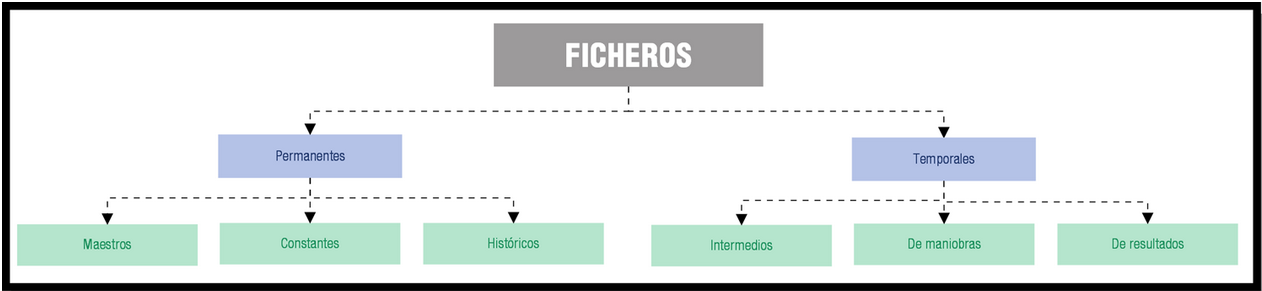
\includegraphics[scale=0.35]{ficheros-tipos.png}
    \caption{Clasificación de ficheros según su función}
\end{figure}

\subsection{Los Soportes de la Información}
Los ficheros se almacenan en soportes de información manejados por periféricos del ordenador, que permiten leer y grabar datos en el soporte. Los soportes más utilizados son las \textbf{cintas magnéticas} y los \textbf{discos} (magnéticos, ópticos o magneto-ópticos).

Al principio se usaban tambores de cinta magnética, similares en tamaño a un disco de vinilo, funcionaban de manera similar a los antiguos casetes, pero al tener un tamaño mucho más grande permitían almacenar mucha mas información, permitiendo el acceso a esta de forma secuencia.

Posteriormente los medios de almacenamiento fueron evolucionando a la par que el hardware, en concreto con la aparición de los disquetes y el disco duro. Estos dispositivos ya permitían el acceso aleatorio a los datos.

Por lo tanto, podemos distinguir dos tipos de dispositivos de almacenamiento de datos:

\begin{itemize}
    \item \textbf{Soportes de Acceso Directo a Datos}: son los más empleados y el acceso a datos se hacer de forma directa, pudiendo colocarlos en la posición que más nos interese.
    \item \textbf{Soporte de Acceso Secuencial}: se suele usar en copias de seguridad y si deseamos leer un dato que esta a mitad de la cinta, tendremos que leer todo lo que hay hasta llegar a esa posición.
\end{itemize}

Si quieres aprender más sobre las características de cintas y discos, puedes consultar los enlaces siguientes:

\begin{itemize}
    \item \href{https://es.wikipedia.org/wiki/Cinta_magn\%C3\%A9tica_de_almacenamiento_de_datos}{Cintas magnéticas de almacenamiento de datos}
    \item \href{https://es.wikipedia.org/wiki/Disco_magn\%C3\%A9tico}{Discos magnéticos} y \href{https://es.wikipedia.org/wiki/Disco_\%C3\%B3ptico}{Discos ópticos}
\end{itemize}

\subsection{Métodos de Acceso a Ficheros}
A medida que la tecnología ha ido evolucionando, el acceso a la información ha ido variando mucho. Los objetivos de fundamentales de estas variaciones son los siguientes:

\begin{itemize}
    \item Proporcionar acceso rápido a los registros.
    \item Conseguir economizar el almacenamiento.
    \item Facilitar la actualización de los registros.
    \item Permitir que la estructura refleje la organización real de la información.
\end{itemize}

Los ficheros se pueden clasificar según como se organiza en la memoria principal, o dicho de otra forma, los métodos de acceso al fichero, que podemos ver en la siguiente figura.

\begin{figure}[ht]
    \centering
    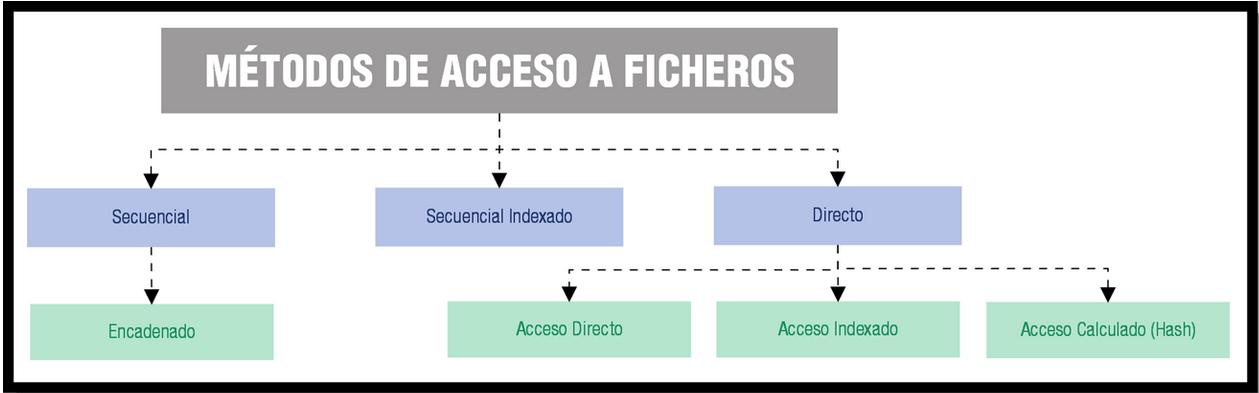
\includegraphics[scale=0.40]{ficheros-acceso.png}
    \caption{Tipos de ficheros por método de acceso}
\end{figure}

Las organizaciones secuencia, de acceso aleatorio o directo e indexado, son las mas comunes. En esta sección vamos a explicar las características de cada uno de los métodos de acceso a ficheros.

\subsubsection{Ficheros Secuenciales}
Un \textbf{fichero secuencial} se caracteriza porque sus registros están almacenados de forma continua, de forma que la única manera de acceder a él, es leyendo un registros detrás de otro hasta el final. En los ficheros secuenciales hay una marca que indica el final del fichero, suele denominarse \textbf{EOF} (End Of File). Así, para detectar el final de fichero solo es necesario encontrar esta marca.

Este tipo de fichero puede usar dispositivos de almacenamiento de acceso secuencial, como cintas magnéticas, aunque también se utilizan en los CD de audio y DVD de vídeo, en los que la música y las imágenes se almacenan en un espiral continua.

Los registros almacenados se identifican por medio de la información ubicada en uno de sus campos, que se denomina \textbf{clave} o \textbf{llave}. Si se ordena un archivo secuencial por su clave es más rápido realizar operaciones sobre el.

\begin{figure}[ht]
    \centering
    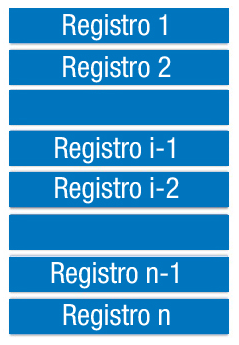
\includegraphics[scale=0.32]{fichero-secuencial.png}
    \caption{Estructura de un fichero secuencial}
\end{figure}

Algunas características de este tipo de ficheros son las siguientes:

\begin{itemize}
    \item La \textbf{lectura} siempre se realiza \textbf{hacia adelante}.
    \item Son ficheros \textbf{monousuario}, no permiten el acceso simultáneo de varios usuarios.
    \item Tiene una \textbf{estructura rígida de campos}. Todos los registros deben aparecer en orden, es decir, la posición de los campos en el registros siempre debe ser la misma.
    \item El \textbf{modo de apertura} del fichero, condiciona la lectura o escritura.
    \item \textbf{Aprovechan al máximo} el soporte de \textbf{almacenamiento}, no dejando huecos vacíos.
    \item Se pueden \textbf{grabar} en \textbf{cualquier tipo} de \textbf{soporte}, tanto secuenciales como direccionales.
    \item Todos los \textbf{lenguajes de programación} contiene instrucciones para \textbf{trabajar} con este tipo de ficheros.
    \item \textbf{No} se pueden \textbf{insertar registros} en los que están \textbf{ya grabados}.
\end{itemize}

\subsubsection{Ficheros de Acceso Directo}
En este tipo de archivos se puede acceder a un registro indicando la posición relativa del registros dentro del archivo, o a través de una \textbf{clave} que forma parte del registro como un \textbf{campo} más. Estos archivos deben almacenarse en dispositivos de memoria masiva con acceso directo como los discos magnéticos.

Cada uno de los registros se guarda en una posición física, que dependerá del espacio disponible en memoria masiva, por lo que la distribución es aleatoria dentro del soporte de almacenamiento. Para acceder a la posición física del registros se utiliza una posición o índice, de forma que no es necesario recorrer todo el fichero para encontrar un determinado registros.

 Esta \textbf{dirección física} se obtendrá tras la aplicación de una \textbf{transformación} específica a la \textbf{clave}. Según como sea esta transformación, existen tres modos de acceso diferente, como podemos ver en la siguiente figura.

\begin{figure}[ht]
     \centering
     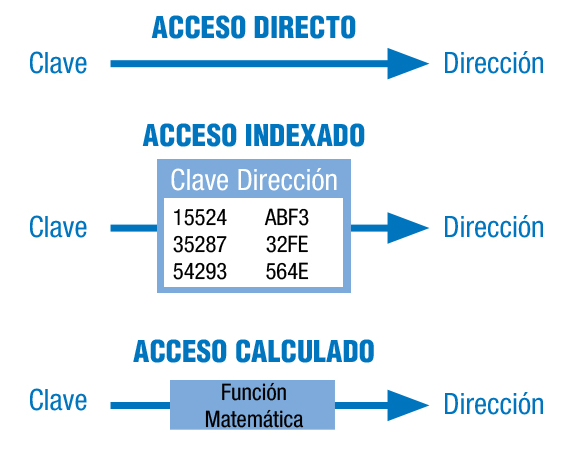
\includegraphics[scale=0.32]{fichero-accesodirecto.png}
     \caption{Modos de acceso a un registro en archivos de acceso directo}
 \end{figure}

El método más rápidos es el \textbf{acceso directo}, donde la clave coincide con la dirección física del registro, teniendo ésta que ser una posición valida dentro del rango de direcciones físicas.

La \textbf{medida de posicionamiento} básico del puntero en el fichero es el \textbf{byte}, dependiendo del tipo de codificación de caracteres que empleemos (\textbf{\gls{Unicode}}, \textbf{\gls{ANSI}}), se usarán 1 o 2 bytes por carácter respectivamente. Teniendo esto en cuenta, el puntero avanza de 1 en 1 o de 2 en 2 bytes para poder leer o escribir cada carácter.

Otras \textbf{características} de este tipo de ficheros son las siguientes:

\begin{itemize}
    \item \textbf{Posicionamiento inmediato}.
    \item \textbf{Registros} de \textbf{longitud fija}.
    \item \textbf{Apertura} del fichero en \textbf{modo mixto}, para lectura y escritura.
    \item Permiten \textbf{múltiples usuarios} al mismo tiempo.
    \item Los \textbf{registros se borran} colocando un cero en la posición que ocupan.
    \item Permiten la utilización de \textbf{algoritmos de compactación} de huecos.
    \item Los archivos se \textbf{crean} con un \textbf{tamaño definido}, es decir, con un máximo de registros definidos durante su creación.
    \item Esta organización solo es posible en \textbf{soportes direccionales}.
    \item Se \textbf{usan} cuando el \textbf{acceso a datos} de un registro se hace siempre empleando la \textbf{misma clave} y la \textbf{velocidad de acceso} al registro es lo que más importa.
    \item Permiten la \textbf{actualización de registros} en el mismo fichero, sin necesidad de copiarlo.
    \item Permiten realizar \textbf{procesos de actualización} en \textbf{tiempo real}.
\end{itemize}

\subsubsection{Ficheros Indexados}
Se basan en el uso de \textbf{indices}, que permiten el acceso a un registros sin tener leer el fichero entero. Estos indices son similares a los de los libros, si nos interesa leer un capítulo podemos recurrir al indice donde se nos dice en que página comienza y acaba dicho capítulo.

Por lo tanto, deberá existir una \textbf{zona de registros} en los que se encuentren los datos del archivo y una \textbf{zona de índices}, que contiene la tabla con las claves de los registros y las posiciones donde se encuentran. La tabla de índices esta ordenada por campos clave.

La tabla de índices será cargada en la memoria principal para realizar en ella la búsqueda de la fila correspondiente a la clave del registros a encontrar, proporcionando así la dirección donde se encuentra el registro. Una vez localizada la dirección, solo es necesario acceder el dispositivo de almacenamiento y colocarlos en la dirección indicada.

\begin{figure}[ht]
    \centering
    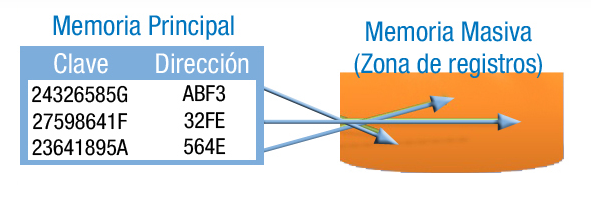
\includegraphics[scale=0.50]{fichero-indexado.png}
    \caption{Ficheros indexados}
\end{figure}

Las características mas relevantes de los ficheros indexados son las siguientes:
\begin{itemize}
    \item El diseño de registros tiene que tener un campo o campos, que permita identificar cada registro de forma única, es decir, no puede haber 2 registros que tengan la misma información en él. A este campo se le llama \textbf{campo clave} y es el que va a servir de índice. Un mismo fichero puede tener varios campos clave, pero al menos uno de ellos \textbf{no puede tener valores duplicados} y se llama \textbf{clave principal}. A las restantes se les llama \textbf{claves alternativas}.
    \item Permite usar el modo de \textbf{acceso secuencial} y el modo de \textbf{acceso directo} para leer la información que guardan sus registros.
    \item Para acceder a estos ficheros usando el modo de \textbf{acceso directo}, se hace conociendo el \textbf{contenido} del \textbf{campo clave} que queremos localizar. Con esta información el sistema operativo puede consultar el índice y conocer la posición dentro del fichero.
    \item Para acceder a este tipo de ficheros usando el m\textbf{modo secuencial}, los registros son \textbf{leídos} por el contenido del \textbf{campo clave}, independientemente del orden en el que fueron grabados, ya que el acceso se hace a través del índice, que para hacer más fácil la búsqueda de registros, permanece siempre ordenado por campos clave.
    \item Solamente puede \textbf{almacenarse} en un \textbf{medio direccionable}, ya que sino no podría usar el modo de acceso directo.
\end{itemize}

\subsubsection{Otros Tipos de Organización}
Además de los tipos de organización de ficheros que ya hemos visto, existen otros como los \textbf{ficheros secuenciales indexados} o los \textbf{ficheros de acceso calculado}, los cuales pasamos a describir a continuación.

\begin{enumerate}[label=(\alph*)]
    \item \textbf{Ficheros Secuenciales Indexados}:

    También llamados parcialmente indexados, al igual que los ficheros indexados existe una \textbf{zona de índices} y otra \textbf{zona de registros de datos}, pero esta última se encuentra \textbf{dividida} en \textbf{segmentos} ordenados.

    En la zona de índices, cada fila hace referencia a cada uno de los segmento. La clave corresponde al último registros del segmento y el índice al registro inicial. Una vez que se accede al primer registro del segmento, dentro de él se localiza (de forma secuencial) el registro buscado.

    Las principales características de este tipo de ficheros son:
    \begin{itemize}
        \item Permite el \textbf{acceso secuencial}. Esto es muy interesante cuando la tasa de accesos es alta. En el acceso secuencial ademas los registros se leen ordenados por el campo clave.
        \item Permite el \textbf{acceso directo a registros}. Realmente \textbf{emula} este tipo de acceso, empleando para ello las tablas de índices. Primero busca la clave en el área de índices y luego va a leer al área de datos en al dirección que indica la tabla.
        \item Se pueden \textbf{actualizar} los \textbf{registros} en el \textbf{mismo fichero}, sin necesidad de crear uno nuevo de copia en el proceso de actualización.
        \item Ocupa \textbf{más espacio} que los \textbf{ficheros secuenciales}, debido al uso del área de índices.
        \item Solo se pueden utilizar \textbf{soportes direccionales}.
        \item Obliga a una \textbf{inversión económica mayor}, por la necesidad de \textbf{programas}, y a veces, \textbf{hardware más sofisticado}.
    \end{itemize}

    \item \textbf{Ficheros de Acceso Calculado o Hash}:

    Cuando usamos ficheros indexados es necesario siempre consultar una tabla para obtener la dirección de almacenamiento a partir de la clave. La técnica de acceso calculado o \textbf{hash}, permite accesos más rápidos, ya que en vez de consultar una tabla utiliza una \textbf{función matemática} (función de hashing) conocida, que a partir de la clave genera la dirección conocida de cada registro. Si la clave el alfanumérica deberá previamente ser transformada en un número.

    El mayor problema que ofrece esta aproximación es que a partir de diferentes claves se puedan obtener la misma dirección de almacenamiento al aplicar la función. A este problema se le denomina \textbf{colisión}, y las claves que generan la misma dirección se denominan \textbf{sinónimos}. Para resolver este problema se aplican diferentes métodos, como tener un bloque de excedentes o zona de sinónimos, o crear un archivo de sinónimos, etc...

    Para llevar a cabo la transformación se existen multitud de métodos, aunque los mas empleados son:

    \begin{itemize}
        \item \textbf{Módulo}: la dirección será igual al resto de la división entera entre la clave y el número de registros.
        \item \textbf{Extracción}: la dirección será igual a una parte de las cifras que se extraen de la clave.
    \end{itemize}

    Una buena función hash, será aquella que produzca el menor número de colisiones. En este caso hay que buscar una función, a poder ser \textbf{\gls{biunivoca}}, que relaciones los posibles valores de la clave con el conjunto de números correlativos de la dirección. Esta función consistirá en realizar una serie de cálculos matemáticos con el valor de la clave hasta obtener un número entre 1 y n, siendo n el número de direcciones que tiene el fichero.
\end{enumerate}

\subsection{Parámetros de Utilización}
En función del uso que se le vaya a dar al fichero, serán convenientes unos u otros métodos de organización. Mediante la utilización de \textbf{parámetros de referencia} podemos determinar el uso de un fichero. Estos parámetros son:

\begin{enumerate}[label=(\alph*)]
    \item \textbf{Capacidad o Volumen}: es el espacio, en caracteres, que ocupa el fichero. La capacidad podrá calcularse multiplicando el número de registros por el tamaño medio de cada registro.
    \item \textbf{Actividad}: permite conocer la cantidad de consultar y modificaciones que se realizan en un fichero. Para poder especificar la actividad hay que tener en cuenta:
    \begin{itemize}
        \item \textbf{Tasa de Consulta o Modificación}: que es el número de registros consultar o modificados en cada tratamiento del fichero, respecto al número total de registros contenidos en él.
        \item \textbf{Frecuencia de Consulta o Modificación}: número de veces que se accede a un fichero para realizar una consulta o modificación en un tiempo predeterminado.
    \end{itemize}

    \textbf{Volatilidad}: mide la cantidad de inserciones y borrados que se efectúan en un fichero. Para determinar la volatilidad es necesario saber:
    \begin{itemize}
        \item \textbf{Tasa de Renovación}: es el tanto por ciento de registros renovados en cada tratamiento del fichero respecto del número de registros totales.
        \item \textbf{Frecuencia de Renovación}: es el número de veces que se accede al fichero para renovarlo durante un período de tiempo determinado.
    \end{itemize}

    \item \textbf{Crecimiento}: es la variación de la capacidad del fichero y se mide con la tasa de crecimiento, que es el porcentaje de registros en los que aumenta el fichero en cada tratamiento.
\end{enumerate}

Teniendo en cuenta estos valores, podremos hacernos una idea de cual es el método de organización que mejor se adapta a nuestra necesidades y cual es el que deberemos usar en nuestros ficheros.

\newpage

\section{Bases de Datos}
Como hemos visto en la sección anterior, los fichero permiten organizar y memorizar conjuntos de datos de un mismo tipo con una determinada estructura, siendo un medio para almacenar la información o resultados de una aplicación. El problema es que si las aplicaciones, al ser diseñadas, dependen directamente de sus archivos, se pierde independencia y surgen serios inconvenientes: como información duplicada, incoherencia de datos, etc...

Aquí es donde aparece el concepto de base de datos. Una \textbf{base de datos} permitirá reunir toda la información relacionada en un único sistema de almacenamiento, pudiendo cualquier aplicación utilizarla de forma independiente y ofreciendo una mejora en el tratamiento de la información.

La gestión de las bases de datos a experimentado gran cantidad de cambios, partiendo de aplicaciones especializadas hasta pasar a convertirse en el núcleo de los entornos informáticos modernos. Con la llegada de internet en los 90, el número de usuario de bases de datos creció exponencialmente, y aunque muchos no sean conscientes de ello, las usan a diario.

Así, conocer los sistemas de gestión de bases de datos, sus conceptos fundamentales, el diseño, lenguajes e implementación de estas, es imprescindible para cualquiera que se este formando en el campo de la informática.

\subsection{Conceptos Básicos}
Una \textbf{base de datos} es una colección de datos relacionados lógicamente entre sí, con una definición y descripción comunes y que están estructurados de una determinada manera. Es un conjunto de datos que representa entidades y sus relaciones, almacenados con la mínima redundancia y posibilitando el acceso a ellos eficientemente por parte de varias aplicaciones.

Las bases de datos no contienen solo los datos de la organización, sino que también almacenan una descripción de dichos datos. Esta descripción es lo que se denomina \textbf{metadatos}, se almacenan en un \textbf{diccionario de datos} o \textbf{catálogo} y es lo que permite la \textbf{independencia de datos} lógico-física.

Una base de datos, constará de los siguientes \textbf{elementos}:
\begin{itemize}
    \item \textbf{Entidades}: objeto real o abstracto, con características diferenciadas de otros, del que se almacena información en la base de datos. En una base de datos de una clínica veterinaria, diferentes entidades podrían ser: ejemplar, doctor, consulta, etc...
    \item \textbf{Atributos}: son los datos que se almacenan en la entidad. Cualquier propiedad o característica puede ser un atributo de una entidad. Continuando con el ejemplo, podrían ser atributos: raza, color, nombre, número de identificación, etc...
    \item \textbf{Registros}: es donde se almacena la información de cada entidad. Es un conjunto de atributos que contienen los datos que pertenecen a una misma repetición de identidad. En nuestro ejemplo un registros podría ser: Podenco, blanco, 121932911, etc...
    \item \textbf{Campos}: donde se almacenan los atributos de cada registro. Teniendo en cuento el ejemplo anterior, un campo podría ser Podenco.
\end{itemize}

El uso de bases de datos ofrece muchas \textbf{ventajas}, entre las que podemos encontrar las siguientes:

\begin{itemize}
    \item \textbf{Acceso Múltiple}: diversos usuarios y aplicaciones podrán acceder a la base de datos sin que existan problemas en el acceso o los datos.
    \item \textbf{Utilización Múltiple}: cada uno de los usuarios o aplicaciones podrá tener una visión única de la base de la estructura de la base de datos, accediendo solo a la parte que le corresponde.
    \item \textbf{Flexibilidad}: la forma de acceso de la información puede ser establecida de diferentes maneras, ofreciendo tiempos de respuesta muy reducidos.
    \item \textbf{Confidencialidad y Seguridad}: el control de acceso de los datos podrá ser establecido para que los usuarios y aplicaciones puedan acceder a unos datos y a otros no, impidiendo a los usuarios no autorizados el uso de la base de datos.
    \item \textbf{Protección Contra Fallos}: en casos de fallos en la información, existen mecanismos bien definidos que permiten la recuperación de los datos de forma fiable.
    \item \textbf{Independencia Física}: un cambio en el soporte físico, por ejemplo un disco duro, no afectaría a los datos o las aplicaciones que acceden a estos.
    \item \textbf{Independencia Lógica}: los datos realizados en la base de datos no afectan a las aplicaciones que acceden a ella.
    \item \textbf{Redundancia}: los datos se almacenan, por lo general, una única vez, aunque si fuera necesario podríamos repetir la información de manera controlada.
    \item \textbf{Interfaz de Alto Nivel}: mediante la utilización de lenguajes de alto nivel puede utilizarse la base de datos de forma sencilla y cómoda.
    \item \textbf{Consulta Directa}: existe una herramienta para poder acceder a los datos de forma interactiva.
\end{itemize}

\subsection{Uso de las Bases de Datos}
Ya sabemos en que consiste una base de datos, ahora veremos que usuarios son los que la utilizan y en que campos se utilizan éstas.

Existen principalmente cuatro \textbf{tipos de personas} que pueden hacer uso de las bases de datos y cada uno de ellos hace un uso diferente de éstas. Estas personas son:

\begin{itemize}
    \item \textbf{El Administrador}

    Es la persona encargada de la creación o implementación física de la base de datos. Es quien escoge los tipos de ficheros, los índices que se deben crear, la ubicación de estos, etc... En general, es quien toma las decisiones del funcionamiento físico del almacenamiento de la información. Además, establecerá la política de seguridad y acceso para garantizar el menos número de problemas.

    \item \textbf{Los Diseñadores}

    Son los encargados de diseñar como será la base de datos. Llevarán a cabo la identificación de los datos, sus relaciones, sus restricciones, etc... Para ello, han de conocer a fondo los datos y procesos que deben representarse en la base de datos. Si estamos hablando de una empresa, deberán conocer la reglas de negocio de esta. Para obtener un buen resultado, el diseñador deberá implicar a todos los usuarios de la base de datos lo antes posible en el proceso.

    \item \textbf{Los Programadores de Aplicaciones}

    Una vez diseñada y construida la base de datos, los programadores se encargarán de implementar los programas de aplicación que servirán a los usuarios finales. Estos programas permitirán la posibilidad de realizar inserciones, actualizaciones o eliminaciones de datos. Para desarrollar estas aplicaciones se utilizan lenguajes de tercera o cuarta generación, como C, FORTRAN, Smalltalk, Ada, Java, etc...

    \newpage

    \item \textbf{Los Usuarios Finales}

    Son los clientes finales de la base de datos. Al diseñar, implementar y mantener la base de datos se busca cumplir con los requisitos establecidos por el cliente para la gestión de su información.
\end{itemize}


Respecto a los \textbf{campos} en los que se\textbf{ usan la bases de datos} y los usos que se les dan son innumerables, aunque en la siguiente lista tienes algunos ejemplos:

\begin{itemize}
    \item Banca: información de clientes, cuentas, transacciones, ...
    \item Líneas Aéreas: información de clientes, vuelos, horarios, ...
    \item Universidades: información de alumnos, asignaturas, profesores, horarios,...
    \item Telecomunicaciones: guardar registros de llamadas realizadas, generar facturas mensuales, mantener saldo de las tarjetas telefónicas y almacenar información sobre las redes.
    \item Medicina: información hospitalaria, biomedicina, genética, ...
    \item Legislación: normativas, registros, etc...
    \item Organismos Públicos: registros de los ciudadanos, certificados, etc...
    \item Justicia y Seguridad: delincuentes, casos, sentencias, investigaciones...
\end{itemize}

Como vemos, prácticamente en cualquier campo en el que se necesite recopilar, almacenar y gestionar información se utilizan las bases de datos.

\subsection{Ubicación de la Información}
Las bases de datos pueden tener un tamaño muy pequeño o ser muy voluminosas, pero independientemente de esto todas se almacenan en discos duros y otros dispositivos de almacenamiento a los que se puede acceder a través de un ordenador. Una base de datos pequeña pueden existir en un archivo pequeño dentro de un disco duro, mientras que una gran base de datos puede necesitar decenas de servidores en diferentes localizaciones.

En esta sección, vamos a ver los tipos de dispositivos y tecnologías de almacenamiento mas utilizados para el despliegue de bases de datos. En la siguiente lista, se detallan estos dispositivos:

\begin{itemize}
    \item \item \textbf{Disco SATA}: es una interfaz de transferencia de datos entre la placa base y algunos dispositivos de almacenamiento como discos duros, lectores o grabadores de CD/DVD, unidades de estado solido u otros dispositivos. La interfaz SATA proporciona mayores velocidades, cables de conexión mas largos, mejor aprovechamiento cuando hay varios dispositivos conectados y capacidad de conectar unidades sin necesidad de apagar el ordenador. La primera generación tenía una tasa de transferencia de 150 MB/s, denominada \textbf{SATA 150 MB/s} o \textbf{Serial-ATA-150}. Actualmente se comercializan dispositivos \textbf{SATA II}, con velocidades de transferencia de 300 MB/s y \textbf{SATA III}, con velocidades de 600 MB/s.

    \item \textbf{Discos SCSI}: son interfaces preparadas para discos de gran capacidad de almacenamiento y gran velocidad de rotación. Se presentan bajo tres especificaciones: \textbf{Standard SCSI}, \textbf{Fast SCSI} y \textbf{Fast-Wide SCSI}. Su velocidad de acceso puede llegar a los 7 ms y la velocidad de transmisión de información secuencia a 5 MB/s, 10 MB/s y 20 MB/s para las versiones Standard, Fast y Fast-Wide respectivamente. Un controlador puede manejar hasta 7 discos duros SCSI.

    \item \textbf{RAID}: acronimo de \textbf{Redundant Array of Independent Disks}, es un contenedor de almacenamiento redundante. Se basa en montar varios discos duros para que trabajen conjuntamente obteniendo mejoras en el almacenamiento, la velocidad, la disponibilidad y la seguridad de la información. Según las características que queramos reforzar se usará una u otra configuración RAID.

    \item \textbf{Sistemas NAS}: es el acrónimo de \textbf{Network Attached Storage}. Estos sistemas de almacenamiento permiten compartir el almacenamiento de un computador (servidor), con ordenadores personales o servidores clientes a través de la red, haciendo uso de un sistema operativo optimizado para dar acceso a los datos a través de protocolos de comunicación específicos. Suelen ser dispositivos de almacenamiento de gran capacidad, varios TeraBytes, generalmente superiores a los discos duros externos y que están conectados con la red.

    \item \textbf{SAN}: acrónimo de \textbf{Storage Area Network}. Se trata de una red concebida, arrays de discos y librerías de soporte. La arquitectura de este tipo de sistema permite que los recursos de almacenamiento estén disponibles para varios servidores en una red de área local o amplia. Debido a que la información almacenada no reside en directamente en ninguno de los equipos de la red, se optimiza el poder de procesamiento para aplicaciones comerciales y la capacidad de almacenamiento se puede proporcionar al servidor que más lo necesite.
\end{itemize}

Aunque no se mencionen en esta lista, en los últimos años la tendencia es usar \textbf{bases de datos en la nube}, que permiten la utilización de bases de datos desarrolladas, implementadas y a las que se accede en un entorno de nube, como una nube privada, pública o híbrida. \cite{cloud01} En la \href{https://www.oracle.com/es/database/what-is-a-cloud-database/}{página de Oracle} puedes encontrar información más detallada sobre este tipo de bases de datos.

\section{Modelos de Bases de Datos}
La clasificación tradicional de las bases de datos establece tres modelos de bases de datos: \textbf{jerárquico}, \textbf{en red} y \textbf{relacional}. En la actualidad el modelo de datos mas empleado es el relacional, aunque hay que tener en cuenta que dos de sus variantes, \textbf{bases de datos distribuidas} y \textbf{orientadas a objetos} son las más empleadas.

En esta sección, vamos a analizar estos modelos de bases de datos así como algunos otros aquí no mencionados.

\subsection{Modelo Jerárquico}
Cuando IBM creó su Sistema Administrado de la Información o IMS, se establecieron las bases para que la gran mayoría de sistemas de gestión de información de los años 70 utilizaran un modelo jerárquico. También recibe el nombre de modelo árbol, ya que utiliza una estructura de árbol invertido para el almacenamiento de los datos.

En el \textbf{modelo jerárquico}, la información se organiza con un jerarquía en el que se establece una relación entre las entidades \textbf{padre/hijo}. De tal forma que existen nodos que contienen atributos o campos y que se relacionan con sus nodos hijos, pudiendo tener cada nodo \textbf{varios hijos}, pero un nodo solo puede tener \textbf{un nodo padre}.

Los \textbf{datos} de este modelo se \textbf{almacenan} en estructuras lógicas llamadas \textbf{segmentos}. Los segmentos se relacionan entre sí usando \textbf{arcos}. Visualmente, este modelo se puede representar como un árbol invertido, estando en la parte superior los padres y en la inferior los hijos.

Hoy en día, debido a sus limitaciones, este modelo esta en desuso. En la siguiente figura podemos ver un ejemplo de estructura jerárquica.

\begin{figure}[ht]
    \centering
    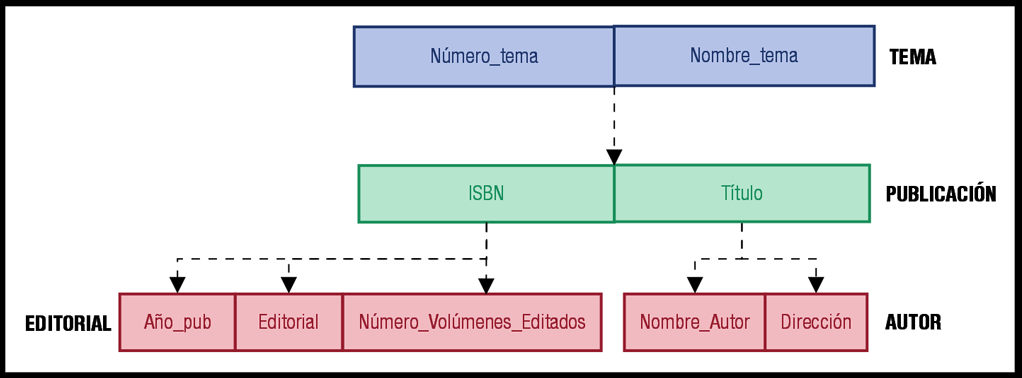
\includegraphics[scale=0.40]{bd-jerarquico.png}
    \caption{Modelo Jerárquico de Bases de Datos}
\end{figure}

\subsection{Modelo en Red}
El modelo de datos en red aparece a mediados de los 60 como respuesta a las limitaciones del modelo jerárquico en cuanto a la representación de relaciones más complejas. Podemos considerar a \textbf{IDS} (Integrated Data Storage) de Bachman como el primer sistema de bases de datos en red. Más adelante, se intento crear un modelo de red por parte de \textbf{\gls{CODASY}}, siendo un modelo que tuvo un gran aceptación a principios de los 70.

El \textbf{modelo en red} organiza la información en \textbf{registros}, también llamados nodos, y \textbf{enlaces}. En los registros se almacenan los datos, mientras que los enlaces permiten relacionar los datos. Las bases de datos en red son parecidas a las jerárquicas, salvo que en éstas un nodo puede tener \textbf{más de un padre}.

En este modelo se puede representar prácticamente cualquier relación de datos, pero su manejo se hace muy complicado. Al no tener que duplicar la información  se ahora en espacio de almacenamiento. El sistema de gestión de la información mas extendido es \textbf{\gls{IDMS}}.

En la siguiente figura podemos ver un ejemplo de este tipo de modelo de bases de datos.

\begin{figure}[ht]
    \centering
    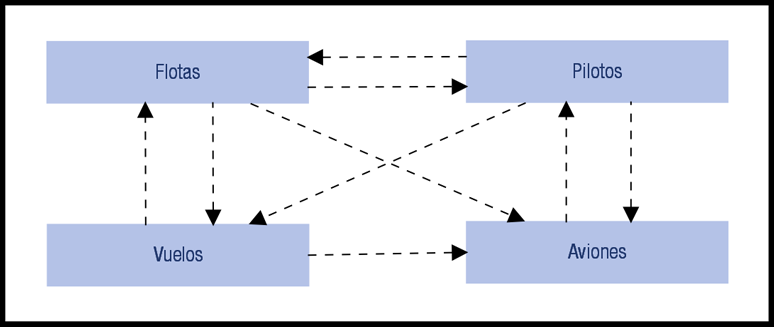
\includegraphics[scale=0.55]{bd-enred.png}
    \caption{Modelo en Red de Bases de Datos}
\end{figure}

\subsection{Modelo Relacional}
Este modelo es posterior a los dos anteriores y fue desarrollado por Codd en 1970. Hoy en día, este tipo de base de datos es la más utilizada.

El \textbf{modelo relacional} es percibida por los usuarios como un conjunto de tablas. Esta percepción es solo a nivel lógico, ya que a nivel físico puede estar implementada mediante diferentes estructuras de almacenamiento. Es modelo utiliza \textbf{tablas bidimensionales} (relaciones) para la representación lógica de los datos y las relaciones entre ellos. Cada relación (tabla) posee un nombre único y contiene un conjunto de columnas.

Cada tabla estará compuesta de los siguientes elementos:

\begin{itemize}
    \item \textbf{Registro/Entidad/Tupla}: es el nombre que recibe cada fila.
    \item \textbf{Campo/Atributo}: es el nombre que recibe cada columna.
    \item \textbf{Clave}: es el atributo o conjunto de estos que identifica de forma única a cada tupla.
\end{itemize}

Al conjunto de valores que puede tomar un atributo se le conoce como \textbf{dominio}. Ademas, las tablas deben cumplir un conjunto de \textbf{requisitos} para que se consideren correctas, que son los siguientes:

\begin{itemize}
    \item Todos los registros son del mismo tipo
    \item La tabla solo puede tener un tipo de registro.
    \item No existen campos o atributos repetidos.
    \item No existen registros duplicados.
    \item No existe orden de almacenamiento de los registros.
    \item Cada registro o tupla debe estar identificada por una clave formada por uno o varios atributos.
\end{itemize}

En la siguiente imagen puedes ver como se relacionan las tuplas y atributos en una base de datos con el modelo relacional.

    \begin{figure}[ht]
    \centering
    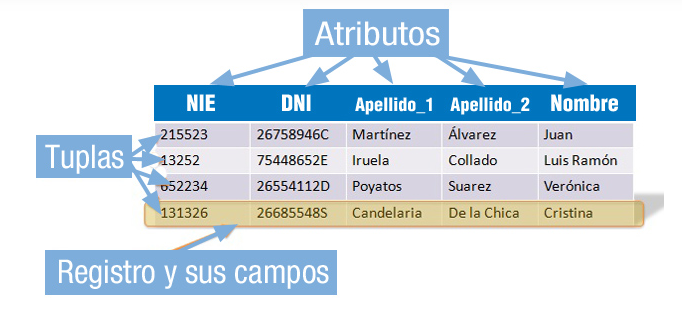
\includegraphics[scale=0.55]{bd-relacional.png}
    \caption{Modelo Relacional de Bases de Datos}
\end{figure}

El lenguaje mas habitual para construir consultas en este tipo de bases de datos es \textbf{SQL} (Structured Query Language), un estándar implementado por los principales motores o sistemas de gestión de bases de datos.

Durante su diseño, una base de datos relacional para por un proceso que se conoce como \textbf{normalización}, que consiste en definir las reglas que determinan las dependencias entre los datos. Si definimos esta dependencia en una base de datos de la forma mas sencilla posible, conseguiremos que la cantidad de espacio necesaria para almacenar los datos sea la menor posible y la facilidad para actualizar la relación sea la mayor posible. Es decir, optimizaremos su funcionamiento.

\subsection{Modelo Orientado a Objetos}
El \textbf{modelo orientado a objetos} define una base de datos en términos de \textbf{objetos}, sus \textbf{propiedades} y sus \textbf{operaciones}. Los objetos con las misma estructura y comportamiento pertenecen a una misma \textbf{clase}, y las clases se organizan en jerarquías. Las operaciones de cada clase se especifican en términos de procedimientos predefinidos denominados \textbf{métodos}. Algunos sistemas existentes en el mercado, basados en el modelo relacional, han sufrido evoluciones incorporando conceptos de la programación orientada a objetos. A estos modelos se les conoce como \textbf{modelos objeto-relacionales}.

El objetivo de este modelo es cubrir las limitaciones del modelo relacional. Gracias a este modelo se incorporan ventajas como la herencia entre tablas, los tipos definidos por el usuario, disparadores almacenables en la base de datos (triggers), soporte multimedia, etc..

En la siguiente imagen, podemos ver un ejemplo del modelo orientado a objetos.

\begin{figure}[ht]
    \centering
    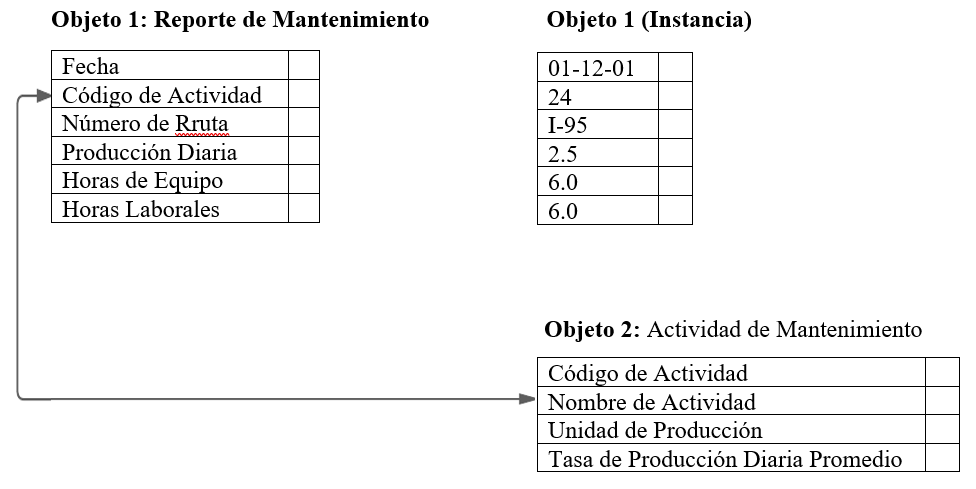
\includegraphics[scale=0.40]{bd-oo.png}
    \caption{Modelo Orientado a Objetos de Bases de Datos}
\end{figure}

Los conceptos más importantes del paradigma de objetos que incorpora el modelo orientado a objetos son los siguientes:

\begin{itemize}
    \item \textbf{Encapsulación}: propiedad que permite ocultar la información al resto de objetos impidiendo así el acceso incorrecto o conflictos.
    \item \textbf{Herencia}: propiedad a través de la cual objetos heredan comportamientos dentro de la jerarquía de clases.
    \item \textbf{Polimorfismo}: propiedad de una operación mediante la cual puede ser aplicada a diferentes tipos de objetos.
\end{itemize}

Desde la aparición de la programación orientados a objetos (OOP) se empezó a pensar en bases de datos adaptadas a estos lenguajes. Este modelo es considerado como el fundamento de las bases de datos de tercera generación, siendo considerara las bases de datos en red como la primera y las relacionales como la segunda generación. Aunque no ha reemplazado a estas últimas, si es el tipo de base de datos que más esta creciendo en los últimos años.

\subsection{Modelo NoSQL}
Las \textbf{bases de datos NoSQL} son bases de datos que no cumplen con el esquema entidad-relación. Tampoco utilizan una estructura de datos de datos en forma de tabla donde se van almacenando los datos, sino que el para el almacenamiento se usan otros formatos como clave-valor, mapeo de columnas, graos, etc...

Esta forma de almacenar los datos tiene ciertas \textbf{ventajas} respecto a los modelos relacionales, las cuales son las siguientes:

\begin{itemize}
    \item Se pueden \textbf{ejecutar} en máquinas con \textbf{pocos recursos}, no requieren apenas computación.
    \item \textbf{Escalabilidad horizontal}: para mejorar el rendimiento de estos sistemas simplemente se consigue añadiendo mas nodos, con la única operación de indicar al sistema cuales son los nodos que están disponibles.
    \item Puede manejar \textbf{gran cantidad de datos}, debido a que usan una \textbf{estructura distribuida} en muchos casos mediante \textbf{tablas Hash}.
    \item \textbf{No generan cuellos de botella}: el principal problema de los sistema SQL es que necesitan transcribir cada sentencia para poder ser ejecutada, lo que constituye a un punto de entrada común, que ante muchas peticiones puede ralentizar el sistema.
\end{itemize}

Después de ver las principales ventajas que tiene el uso de este modelo, en la siguiente lista vemos las principales \textbf{diferencias} que nos podemos encontrar entre las bases de datos \textbf{NoSQL} y los sistemas \textbf{SQL} son las siguientes:

\begin{itemize}
    \item \textbf{No utilizan SQL} como lenguaje de consulta. La mayoría de bases de datos NoSQL evitan usar este lenguaje o, como mucho, lo usan como apoyo.
    \item \textbf{No utilizan} estructuras fijas como \textbf{tablas} para el almacenamiento de datos. Permiten hacer uso de otros sistemas de almacenamiento de información como clave-valor, objetos o grafos.
    \item \textbf{No} suelen permitir \textbf{operaciones JOIN}. Al disponer de un volumen de datos tan extremadamente grande cuando la operación no es la búsqueda de una clave, la sobrecarga puede llegar a ser muy costosa. La solución en este caso sería desnormalizar los datos, o bien realizar el JOIN mediante software en la capa de aplicación.
    \item \textbf{Arquitectura distribuida}: las bases de datos relacionales suelen estar centralizas en una misma máquina o bien en una estructura master-slave, sin embargo en los casos NoSQL la información puede estar compartida por varias máquinas mediante mecanismos de tablas Hash distribuidos.
\end{itemize}

Como hemos comentado, este modelo de bases de datos no usa tablas para almacenar datos, sino que se emplean otros tipos de almacenamiento que no suelen usar en bases de datos relacionales. Así, dependiendo del \textbf{tipo de almacenamiento} que se use en una base de datos NoSQL, estas puede pueden clasificarse en:

\begin{enumerate}[label=(\alph*)]
    \item \textbf{Bases de datos clave-valor}: es el modelo de bases de datos NoSQL más popular, además de ser el más sencillo en cuanto a funcionalidad. En este tipo de sistemas, cada elemento está identificado por una \textbf{llave única}, lo que permite la recuperación de información de una forma muy rápida. Información que habitualmente esta almacenada como un \textbf{objeto binario} (BLOB). Se caracterizan por ser \textbf{muy eficientes} tanto para las \textbf{lecturas} y las \textbf{escrituras}. Algunos ejemplos de estas bases de datos son Cassandra, BigTable o HBase.

    \item \textbf{Bases de datos documentales}: estas bases de datos almacenan la información como un documento, por norma general con una estructura simple como \textbf{JSON} o \textbf{XML} y donde se utiliza una \textbf{clave única} para cada registro. Es tipo permite, ademas de realizar búsquedas por clave-valor, realizar consultar más avanzadas sobre el contenido del documento. Son las bases de datos NoSQL \textbf{más versátiles}. Se pueden utilizar en muchos tipos de proyectos, incluso en muchos que tradicionalmente usarían bases de datos relacionales. Algunas de las mas utilizadas son MongoDB o CouchDB.

    \item \textbf{Bases de datos en grafo}: en este tipo de bases de datos, la información se presenta como nodos en un grafo y sus relaciones como aristas, de manera que se puede hacer uso de la teoría de grafos para recorrerla. Este tipo de bases de datos ofrece una navegación más eficiente que las bases de datos relacionales. Algunos ejemplos de estas bases de datos son Neo4j, InfoGrid o Virtuoso.
\end{enumerate}

Como vemos, hay diferentes clases de bases de datos NoSQL, cada una con sus características propias, con sus ventajas e inconveniente. Dependiendo de nuestras necesidades, podemos elegir una u otra, pero en la actualidad hay unas pocas \textbf{bases de datos NoSQL} que son las \textbf{más usada} y que son las siguientes:

\begin{itemize}
    \item \textbf{Cassandra}: se trata de una base de datos creada por \textbf{Apache} y que esta basada en el modelo \textbf{clave-valor}. Dispone de un lenguaje propio para realizar la consultas, \textbf{CQL} (Cassandra Query Language). Cassandra esta desarrollada en Java, por lo que puede correr en cualquier sistema que tenga una JVM.

    \item \textbf{Redis}: se trata de una base de datos tipo \textbf{calve-valor}. Se puede imaginar como un array gigante en memoria para almacenar datos, los cuales pueden ser cadenas, hashes, conjuntos de datos o listas.

    \item \textbf{Mongo DB}: se trata de una base de datos \textbf{orientada a documentos} de \textbf{esquema libre}, es decir, cada entrada puede tener un esquema de datos diferente que nada tenga que ver con el resto de registros almacenados. Es bastante rápida a la hora de ejecutar sus operaciones ya que esta desarrollada en C++. Es una de las bases NoSQL favoritas de los desarrolladores.

    \item \textbf{CouchDB}: se trata de un sistema desarrollado por \textbf{Apache} y que funciona sobre sistemas \textbf{Linux} y \textbf{OSX}, pero no sobre Windows. Utiliza Javascript como principal lenguaje de interacción. Permite la creación de \textbf{vistas}, un mecanismo para crear combinaciones para retornar valores de varios documentos, es decir, CouchDB permite operaciones \textbf{JOIN} típicas de las bases de datos relacionales.
\end{itemize}

Como vemos hay mucha variedad de bases de datos NoSQL, si quieres ampliar información puedes consultar este blog sobre \href{http://basesdedatosnosql.blogspot.com/}{Bases de Datos NoSQL} o este artículo sobre las \href{https://www.ondho.com/claves-para-elegir-tu-base-de-datos-nosql/}{claves para elegir tu BD NoSQL}.


\subsection{Otros Modelos}
Además de las bases de datos que ya hemos visto, existen otros modelos, que aunque no vamos a ver con tanta profundidad, son dignos de mención. Estos modelos, que en algunos casos son un evolución de los ya vistos, son los siguientes:

\begin{itemize}
    \item \textbf{Modelo Objeto-Relacional}

    Las bases de datos que pertenecen a este modelo, son un híbrido entre el modelo de bases de datos relacional y el orientado a objetos. El principal inconveniente de las bases de datos orientadas a objetos es el coste de la conversión de las bases de datos relacionales a estas.

    En una \textbf{base de datos objeto-relacional} (BDOR) siempre se busca obtener lo mejor del modelo relacional, incorporando las mejoras ofrecidas por la orientación a objetos. En este modelo se siguen almacenando tuplas, aunque la estructura de las tuplas no esta restringida sino que las relaciones pueden ser definidas en función de otras,  que es lo que denominamos herencia directa.

    El estándar en el que se basa este modelo es el \textbf{\gls{SQL99}}. Este estándar ofrece la posibilidad de añadir a las bases de datos relacionales procedimientos almacenados de usuarios, triggers, tipos definidos por el usuario, consultar recursivas, bases de datos \textbf{\gls{OLAP}}, etc...

    También permite añadir funciones que tengan código en algún lenguaje de programación como SQL, Java, C, etc...

    La mayoría de bases de datos relacionales clásicas de gran tamaño, como Oracle, SQL Server, etc.., son objeto-relacionales.


    \item \textbf{Modelo de Bases de Datos Deductiva}

    Es modelo de bases de datos almacena la información y permite hacer deducciones a través de \textbf{inferencias}. Es decir, se derivan nuevas informaciones a partir de las que se han introducido explícitamente en la base de datos por parte del usuario.

    Las \textbf{bases de datos deductivas} son también llamadas bases de datos lógicas, al basarse en lógica matemática. Surgieron para contrarrestar las limitaciones del modelo relacional para las respuesta a consultas recursivas y la deducción de relaciones indirectas entre los datos almacenados.

    \item \textbf{Modelo de Bases de Datos Multidimensionales}

    Son bases de datos ideadas para desarrollar aplicaciones muy concretas. Básicamente almacena sus datos con varias dimensiones, es decir que en vez de un valor, encontramos varios dependiendo de los ejes definidos o una base de datos de estructura basada en dimensiones orientada a consultas complejas y alto rendimiento. En una base de datos multidimensionales, la información se representa como matrices multidimensionales, cuadros de múltiples entradas o funciones de varias variables sobre conjuntos finitos. Cada una de estas matrices se denomina cubo. Eso facilita el manejo de grandes cantidades de datos dentro de las empresas, dándole a esto una amplia aplicación dentro de varias áreas y diferentes campos del conocimiento humano.

    \item \textbf{Modelo de Bases de Datos Transaccionales}

    Son bases de datos caracterizadas por su velocidad para gestionar el intercambio de información, se utiliza sobre todo en sistemas bancarios, análisis de calidad y datos de producción industrial. Son bases de datos muy fiables, ya que en ellas cada una de las operaciones de inserción, actualizado o borrado se realizan completamente o se descartan.
\end{itemize}

\section{Tipos de Bases de Datos}
Como hemos visto, según el modelo de datos las bases de datos se pueden clasificar en diferentes tipos. Pero este no es la única clasificación de bases de datos que existe. Atendiendo a diferentes características y criterios, las bases de datos se pueden clasificar en los siguientes tipos:


\begin{enumerate}[label=(\alph*)]
    \item \textbf{Bases de datos según su contenido}

    Las bases de datos se pueden clasificar según el tipo de contenido que albergan, en este caso las bases de datos pueden ser:

    \begin{itemize}
         \item \textbf{Bases de datos con información actual}: contienen información muy concreta y actualizada, normalmente, de tipo numérico: estadísticas, series históricas, resultados de encuestas, convocatorias de becas, ofertas de empleo, etc...

         \item \textbf{Directorios}: recogen datos sobre personas o instituciones especializadas en una actividad o materia concreta. Hay directorios de profesionales, de investigadores, de centros de investigación, de bibliotecas, etc...

          \item \textbf{Bases de datos documentales}: en este tipo, cada registro se corresponde con un documento, sea este de cualquier tipo: publicación impresa, documento audiovisual, gráfico, etc... Dependiendo de si incluye o no 	el contenido completo de los documentos que describen, podemos tener:
            \begin{itemize}
                \item \textbf{Bases de datos de texto completo}: constituidas por los propios documentos en formato electrónico, por un volcado completo de los datos.

                \item \textbf{Archivos electrónicos e imágenes}: constituidas por referencias que permiten el enlace directo con la imagen del documento original, sea este un documento iconográfico o un documento impreso digitalizado en forma de imagen.

               \item \textbf{Bases de datos referenciales}: sus elementos no contienen el texto original, sino tan sólo información fundamental para describir y permitir la localización de los documentos impresos, sonoros, iconográficos, audiovisuales o electrónicos. En este sistema de información solo se pueden obtener referencias sobre documentos que habrá que localizar en otro servicio.
        \end{itemize}
    \end{itemize}

    \item \textbf{Bases de datos según su uso}

    Las bases de datos también se puede clasificar según el número de usuario que la usen. Así, una base de datos puede ser:

    \begin{itemize}
        \item \textbf{Base de datos individual}: es una base de datos utilizada, básicamente, por una sola persona. El sistema administrador de base de datos y los datos son controlados por el mismo usuario. Puede estar almacenada en la unidad de disco duro del usuario o en el servidor de archivos de una red de área local. Por ejemplo, un gerente podría tener una base de datos para el control de sus vendedores y su desempeño.

        \item \textbf{Bases de datos compartida}: son bases de datos con múltiples usuarios y que probablemente pertenezcan a la misma organización, como la base de datos de una compañía. Se encuentra alojada en una computadora potente y bajo el control de un profesional en el área, el administrador de bases de datos. Los usuarios tienen acceso a la base de datos mediante una red de área local o área extensa.

        \item \textbf{Bases de datos de acceso público}: son bases de datos accesibles por cualquier persona. Puede no ser necesario pagar un canon para hacer uso de los datos contenidos en ellas.

        \item \textbf{Bases de datos propietarias o bancos de datos}: se tratan de bases de datos de gran tamaño y desarrolladas por una organización para contener información sobre temas especializados o de carácter particular. El público general puede tener acceso a estas bases de datos a veces de forma gratuita y otras pagando una cuota. Pueden ofrecer información que va desde negocios, economía, inversión, técnica y científica hasta servicios de entretenimiento.
    \end{itemize}

    \item \textbf{Bases de datos según la variabilidad de la información}

    La variabilidad de la información, es decir, si la información almacenada es estática o dinámica, es otro criterio por el que podemos clasificar las bases de datos. Siendo estas:

    \begin{itemize}
        \item \textbf{Bases de datos estáticas}: son bases de datos de sólo lectura. Se utilizan para el almacenamiento de datos históricos que pueden ser analizados y utilizados para el estudio del comportamiento de un conjunto de datos a través del tiempo. Permite realizar proyecciones y toma de decisiones.

        \item \textbf{Bases de datos dinámicas}: son bases de datos donde la información almacenada se modifica con el tiempo, permitiendo operaciones como actualización y adición de datos, además de operaciones fundamentales de consulta.
    \end{itemize}

    \item \textbf{Bases de datos según la localización de la información}

    Las bases de datos se pueden clasificar también según como tienen distribuida su información, pudiendo ser:

    \begin{itemize}
    \item \textbf{Bases de datos centralizadas}: son bases de datos ubicada en un único lugar, un único computador. Pueden ser sistemas monousuario que se ejecutan en un ordenador o sistemas de bases de datos de alto rendimiento que se ejecutan en grandes sistemas. Este tipo de organización facilita el mantenimiento, sin embargo, hace que la información almacenada en dicha base de datos sea más vulnerable a fallos y limita su acceso. Este tipo de bases de datos puede ofrecer dentro de la arquitectura Cliente/Servidor dos configuraciones:

    \begin{itemize}
        \item \textbf{Basada en el anfitrión}: ocurre cuando la máquina cliente y servidor son la misma. Los usuarios se conectarán directamente a la máquina donde se encuentra la base de datos.

        \item \textbf{Basa en cliente/servidor}: ocurre cuando la base de datos reside en una máquina servidor y los usuarios acceden a la base de datos desde su máquina cliente a través de la red.
    \end{itemize}

    \item \textbf{Bases de datos distribuidas}: una base de datos distribuida consiste en un sistema de bases de datos formado por diferentes bases de datos situadas en diferentes espacios físicos o lógicos y conectadas mediante redes. Los usuarios utilizan estas bases de datos mediante una variedad de redes de comunicación. Un ejemplo, sería una empresa con diferentes centros regionales, cada uno con su base de datos, pero donde los gerentes pueden acceder a estas como si fuera una única base de datos.
    \end{itemize}

    \item \textbf{Bases de datos según el órgano productos}

    También se pueden clasificar las bases de datos según quien sea el productos de la información alojada en ésta. Podemos encontrar los siguientes tipos:

    \begin{itemize}
       \item \textbf{Bases de datos de organismos públicos y de la administración}: las bibliotecas y centros de documentación de los ministerios, instituciones públicas, universidades y organismos de investigación públicos, entre otros, generan gran cantidad de información. Estos sistemas pueden ser:

       \begin{itemize}
          \item Bases de datos de acceso público, sean gratuitas o no.
          \item Bases de datos de uso interno, con información de acceso restringido.
       \end{itemize}

       \item \textbf{Bases de datos de instituciones sin ánimos de lucro}: fundaciones, asociaciones, sindicatos y organizaciones no gubernamentales elaboran frecuentemente sus propios sistemas de información especializados.

       \item \textbf{Bases de datos de entidades privadas o comerciales}: los centros de documentación, bibliotecas y archivos pueden elaborar diferentes tipos de sistemas de información:
       \begin{itemize}
           \item Bases de datos de uso interno para facilitar la circulación de la información dentro de la empresa.
           \item Bases de datos de uso interno que ocasionalmente ofrecen servicios hacia el exterior.
           \item Bases de datos comerciales, diseñadas específicamente para ser usadas por usuarios externos.
       \end{itemize}

    \item \textbf{Bases de datos realizadas por cooperación en red}: se trata de sistema de información cuya elaboración es compartida por diversas instituciones, bases de datos internacionales que se elaboran a través de este sistema de trabajo, con diversos centros nacionales responsables de la información perteneciente a cada país.
    \end{itemize}

    \newpage

    \item \textbf{Bases de datos según su modo de acceso}

    Otra forma de clasificar las bases de datos es atendiendo al modo en el que se accede a ellas, como puede ser:

    \begin{itemize}
       \item \textbf{Bases de datos de acceso local}: pasa consultar es necesario acudir al organismo productor, a su biblioteca o archivo. Pueden ser consultadas en monopuesto en varios puntos de la red local.

        \item \textbf{Bases de datos en CD-ROM}: pueden adquirirse por compra o suscripción bien directamente por un particular o por una biblioteca o centro de documentación que permita su consulta a sus usuarios. En algunas instituciones se instalan diferentes CD-ROMs en una red local para permitir su consulta desde cualquier ordenador conectado a dicha red.

        \item \textbf{Bases de datos en línea}: pueden consultarse desde cualquier ordenador conectado a internet. La consulta puede ser libre o exigir la solicitud previa de una clave personal de entrada, llamado password. Hay diferentes tipos de acceso en línea:
        \begin{itemize}
            \item \textbf{Acceso vía telnet o mediante internet}: el usuario realiza una conexión estable al host (anfitrión) en donde se halla la base de datos, a través de internet. La interfaz de usuario instalada en el host determinará si la consulta debe hacerse por menús, comandos o expresión en un lenguaje determinado. Cuando un usuario accede vía telnet, inicia una sesión interactiva con el programa que gestiona la base de datos, que le permite realizar todas las posibles consultas que soporte el sistema: selección, combinación y visualización o impresión de resultados. En cualquier momento podrá visualizar todas las consultas realizadas hasta ese momento y establecer combinaciones entre ellas.

            \item \textbf{Acceso vía Web}: conexión a través de un formulario existente en una página web, diseñado para realizar consultas en la base de datos.
        \end{itemize}

        Una misma \textbf{base de datos} puede tener \textbf{diferentes formas de acceso}, por ejemplo, puede tener acceso local y ademas una edición en CD-ROM y un acceso en línea. Sin embargo, puede haber diferencias entre el contenido al que se puede acceder por cada vía o el grado de actualización de la información.
    \end{itemize}

    \item \textbf{Bases de datos según cobertura temática}

    Por último, podemos clasificar las bases de datos según el tema de la información que contiene y la cobertura de este. Atiendo a este criterio podemos encontrar los siguientes tipos de bases de datos:

    \begin{itemize}
        \item \textbf{Bases de datos científico-tecnológicas}: contienen información destinada a los investigadores de cualquier ámbito científico o técnico. A su ves, este grupo puede subdividirse en:

        \begin{itemize}
            \item \textbf{Bases de datos multidisciplinares}. abarcan varias disciplinas científicas o técnicas.
            \item \textbf{Bases de datos especializadas}: recopilan y analizan documentos pertenecientes a una disciplina concreta: biomedicina, farmacéutica, química, etc...
        \end{itemize}

        \item \textbf{Bases de datos económico-empresariales}: contienen información de interés para empresas y entidades financieras...

        \item \textbf{Bases de datos de medios de comunicación}: contienen información de interés para profesionales de los medios de comunicación de masas: prensa, radio, televisión...

        \item \textbf{Bases de datos de ámbito político-administrativo y jurídico}: contienen información para los organismos de la administración y los profesionales de derecho: legislación, jurisprudencia, etc...

        \item \textbf{Bases de datos de ámbito sanitario}: además de las propias pertenecientes al primera grupo de bases de datos científicas, existen otras de interés en este sector: historiales médicos, archivos hospitalarios, etc...

        \item \textbf{Bases de datos para el gran público}: contienen información destinada a cubrir necesidades de información general, de interés para gran número de usuarios.
    \end{itemize}
\end{enumerate}

\section{Sistemas Gestores de Bases de Datos}
Para poder tratar la información contenida en las bases de datos se utilizan sistemas gestores de bases de datos, o SGBD, también llamados DBMS (DataBase Management System), que ofrece un conjunto de aplicaciones que permiten acceder y gestionar dichos datos.

Un \textbf{Sistema Gestos de Bases de Datos}, es el conjunto coordinado de programas, procedimientos, lenguajes, etc.., que suministra, tantos a los usuarios no informáticos como a los analistas programadores, o al administrador,  los medios necesarios para describir y manipular los datos contenidos en una base de datos, manteniendo su integridad, confidencialidad y seguridad.

El SGBD permite a los usuarios la creación y mantenimiento de una base de datos, facilitando la definición construcción y manipulación de la información contenida en éstas. La \textbf{definición} de una base de datos consistirá en especificar los tipos de datos, las estructuras y las restricciones que los datos han de cumplir a la hora de almacenarse en dicha base de datos. Por otro lado, la \textbf{construcción} una base de datos será el proceso de almacenamiento de datos concreto en un medio o soporte de almacenamiento que esté supervisado por el SGBD. Finalmente, la \textbf{manipulación} de la base de datos incluirá la posibilidad de realización de consultas para recuperar documentación específica, la actualización de datos y la generación de informes a partir de su contenido.

El uso de un SGBD ofrece muchas suscripción \textbf{ventajas} a la hora de gestionar una base de datos, algunas de ellas son las siguientes:

\begin{itemize}
    \item Proporcionar al usuario una \textbf{visión abstracta} de los \textbf{datos}, ocultando la complejidad relacionada con como se almacenan dichos datos.

    \item Ofrecen \textbf{independencia física}, es decir, la visión que tiene el usuario de la información y la manipulación de los datos almacenados en la base de datos, es independiente de como estén almacenados físicamente.

    \item Disminuye la \textbf{\gls{redundancia}} y la \textbf{\gls{inconsistencia}} de datos.

    \item Asegura la \textbf{\gls{integridad}} de los datos.

    \item \textbf{Facilitan} el \textbf{acceso a datos}, aportando rapidez y evitando la perdida de datos.

    \item \textbf{Aumenta} la \textbf{seguridad} y \textbf{privacidad} de los datos.

    \item Mejoran la \textbf{eficiencia}.

    \item Permite compartir datos y \textbf{accesos concurrentes}.

    \item Facilita el \textbf{intercambio de datos} entre \textbf{diferentes sistemas}.

    \item Incorpora mecanismos de \textbf{copia de seguridad} y \textbf{recuperación} de datos para restablecer la información en caso de fallo.
\end{itemize}

El SGBD interacciona con otros elementos software del sistema, en concreto con el sistema operativo. Los datos almacenados de forma estructurada en la base de datos son usados por otras aplicaciones, será el SGBD quien ofrecerá una serie de facilidades a éstas para el acceso y manipulación de la información, basándose en métodos y funciones propias del sistema operativo.

\subsection{Funciones de SGBD}
Un SGBD realiza tres funciones principales, como es la descripción, manipulación y utilización de los datos. A continuación se detalla cada una de estas funciones.

\begin{enumerate}
    \item \textbf{Descripción}

    Permite al diseñador de base de datos crear las estructuras adecuadas para integrar los datos. Esta función es la que permite definir las tres estructuras de la base de datos: \textbf{Estructura interna}, \textbf{Estructura conceptual} y \textbf{Estructura externa}.

    Esta función se lleva a cabo mediante el \textbf{lenguaje de descripción de datos} o \textbf{DDL}. Mediante este lenguaje, se definen la estructuras de datos, relaciones entre estos y las restricciones que deben cumplir.

    Se especificarán las características de los datos a cada uno de los tres niveles:

    \begin{itemize}
        \item \textbf{A nivel interno} (estructura interna), se ha de indicar el espacio de disco reservado para la base de datos, la longitud de los campos, su modo de presentación, etc...

        \item \textbf{A nivel conceptual} (estructura conceptual), se proporcionan herramientas para la definición de identidades y su identificación, atributos de las mismas, interrelación entre ellas, restricciones de integridad, etc.., es decir, el esquema de la base de datos.

        \item \textbf{A nivel externo} (estructura externa), se deben definir la vistas de los diferentes usuarios  través del lenguaje para la definición de estructuras externas. Además el SGBD se encargará de la transformación de las estructuras externas orientadas al usuario a las estructura conceptuales y de la relación de esta con la estructura física.
    \end{itemize}

    \item \textbf{Manipulación}

    Permite a los usuarios de la base de datos buscar, modificar, añadir o suprimir los datos de la misma, siempre de acuerdo con las normas de seguridad dictadas por el administrador. Se llevará a cabo mediante un \textbf{lenguaje de manipulación de datos} o \textbf{DML} que facilita los instrumento necesarios para la realización de estas tareas.

    También se encarga de definir \textbf{la vista externa} de todos lo usuarios de la base de datos o vistas parciales que cada usuario tiene de los datos definidos con el DDL.

    Por manipulación podemos entender:

    \begin{itemize}
        \item La recuperación de información almacenada en la base de datos, conocida como \textbf{consulta}.
        \item La \textbf{inserción} de nueva información.
        \item El \textbf{borrado} de información almacenada.
        \item La \textbf{modificación} de la información de la base de datos.
    \end{itemize}


    \item \textbf{Control}

    Permite al administrador de la base de datos establecer mecanismos de protección de las diferentes visiones de los datos asociadas a cada usuario, proporcionando elementos de creación y modificación de dichos usuarios. Adicionalmente incorpora sistema de creación de copias de seguridad, carga de ficheros, auditoría, protección contra ataques, configuración del sistema, etc...

    El lenguaje que implementa esta función es el \textbf{lenguaje de control de datos} o \textbf{DCL}.
\end{enumerate}

Para de desarrollar todas estas funciones, usaremos el \textbf{Lenguaje Estructurado de Consultas} o \textbf{SQL} (Structured Query Language). Este lenguaje proporciona sentencias para la realización de operaciones DDl, DML, y DLC.

SQL fue publicado por ANSI en 1986 y ha ido evolucionando a lo largo del tiempo. Además, los SGBD suelen proporcionar otras herramientas que complementan a estos lenguajes como generadores de formularios, informes, interfaces gráficas, generadores de aplicaciones, etc...

\subsection{Componente de un SGBD}
Un SGBD es un paquete de software complejo que ha de proporcionar servicios relacionados con el almacenamiento y la explotación de los datos de forma eficiente. Para realizar esto, incluyendo las funciones vistas en el punto anterior, cuenta con un conjunto de componentes, que son los siguientes:

\begin{enumerate}
    \item \textbf{Lenguajes de la base de datos}

    Cualquier SGBD ofrece la posibilidad de usar lenguajes e interfaces adecuadas para los diferentes usuarios. A través de los lenguajes se pueden especificar los datos que componen la base de datos, su estructura, relaciones, reglas de integridad, control de acceso, características físicas y vistas externas de los usuarios.

    Los lenguajes del SGBD son:

    \begin{itemize}
        \item Lenguaje de Definición de Datos (\textbf{DDL})
        \item Lenguaje de Manejo de Datos (\textbf{DML})
        \item Lenguaje de Control de Datos (\textbf{DCL})
    \end{itemize}

    \item \textbf{Diccionario de Datos}

    Descripción de los datos almacenados. Se trata de información útil para los programadores de aplicaciones. Contiene la información lógica de las estructuras que almacenan los datos, su nombre, descripción, contenido y organización. En una base de datos relacional, el diccionario de datos aportará información sobre:

    \begin{itemize}
        \item Estructura lógica y física de la BD.
        \item Definición de tablas, vistas, índices, disparadores, procedimientos, funciones, etc...
        \item Cantidad de espacio asignado y utilizado por los elementos de la BD.
        \item Descripción de las restricciones de integridad.
        \item Información sobre los permisos asociados a cada perfil de usuario.
        \item Auditoría de acceso a datos, utilización, etc...
    \end{itemize}

    \item \textbf{El Gestor de Base de Datos}

    Es la parte del software encargada de garantizar el correcto, íntegro, seguro y eficiente acceso y almacenamiento de los datos. Es componente es el encargado de proporcionar una interfaz entre los datos almacenados y los programas de aplicación que los manejan. Es un intermediario, entre el usuario y los datos. También es el encargado de garantizar la seguridad, privacidad e integridad de los datos, controlando los accesos concurrentes e interactuando con el sistema operativo.

    \item \textbf{Usuarios de la Base de Datos}

    En un SGBD existen diferentes tipos de usuarios, cada uno de ellos con una serie de permisos sobre los objetos de la base de datos. Generalmente, existirán los siguientes usuarios:

    \begin{itemize}
        \item El \textbf{administrador} de la base de datos o \textbf{Database Administrator} (DBA), que será la persona o conjunto de ellas encargadas de la administración de la base de datos. Tiene el control centralizado de la base de datos y es el responsable de su buen funcionamiento. Se encarga de autorizar el acceso a la base de datos, de coordinar y vigilar su utilización y de adquirir los recursos software y hardware necesarios.

        \item Los \textbf{usuarios} de la base de datos, que serán de diferentes tipos y con diferentes necesidades sobre los datos, así como con diferentes accesos y privilegios. Podemos hacer la siguiente clasificación:

        \begin{itemize}
            \item Diseñadores
            \item Operadores y personal de mantenimiento.
            \item Analistas y programadores de aplicaciones.
            \item Usuarios finales: casuales, simples, avanzados y autónomos.
        \end{itemize}
    \end{itemize}

    \item \textbf{Herramientas de la Base de Datos}

    Son un conjunto de aplicaciones que permiten al administrador la gestión de la base de datos, de los usuarios y permisos, generadores de formularios, informes, interfaces gráficas, etc...
\end{enumerate}

\subsection{Arquitectura de un SGBD}
Un SGBD tiene una arquitectura que simplifica a los diferentes usuarios de la base de datos su labor. El objetivo fundamental es separar los programas de aplicación de la base de datos física.

Encontrar un estándar para estar arquitectura no es una tarea sencilla, aunque los tres estándares más importantes en el campo de las bases de datos son \textbf{ANSI/SPARC/X3}, \textbf{CODASYL} y \textbf{ODMG}, este último solo para bases de datos orientadas a objetos. Tanto ANSI (EEUU) como ISO (internacional), son el referente en cuanto a estandarización de bases de datos, conformando un único modelo de bases de datos.

La arquitectura propuesta proporciona tres niveles de abstracción: \textbf{nivel físico}, \textbf{nivel lógico o conceptual} y \textbf{nivel externo o visión del usuario}. La características de cada uno de estos niveles son las siguientes:

\begin{itemize}
    \item \textbf{Nivel físico}: En este nivel se describen la estructura física de la base de datos a través de un esquema interno encargado de detallar el sistema de la base de datos y sus métodos de acceso. Es el nivel más cercado al almacenamiento físico. A través del esquema físico se indica, entre otras cosas, los archivos que contienen la información, su organización, los métodos de acceso a registros, los tipos de registros, la longitud, etc...

    \item \textbf{Nivel lógico}: En este nivel se describe la estructura completa de la base de datos a través de un esquema que detalla entidades, atributos, relaciones, operaciones de los usuarios y restricciones. Los detalles del almacenamiento se ocultan, permitiendo una abstracción a más nivel.

    \item \textbf{Nivel externo}: En este nivel se describen las diferentes vistas que los usuarios tendrán de la base de datos. Cada grupo de usuarios verá sólo la parte de la base de datos que le interesa, ocultando el resto.
\end{itemize}

Para una base de datos, existirá solo un esquema interno, uno lógico y podrían existir varios esquemas externos definidos para uno o varios grupos de usuarios.

Gracias a esta arquitectura se consigue \textbf{independencia de datos} a dos niveles:
\begin{itemize}
    \item \textbf{Independencia Lógica}: podemos modificar el esquema conceptual sin alterar los esquemas externos ni los programas de aplicación.

    \item \textbf{Independencia Física}: podemos modificar el esquema interno sin alterar el esquema lógico ni los externos. Es decir, se puede cambiar el sistema de almacenamiento, reorganizar ficheros, añadir nuevos, etc.., si que esto afecte al resto de esquemas.
\end{itemize}

Esta arquitectura, como hemos visto, tiene muchas ventajas, siendo la empleada en la mayoría de SGBD. En la siguiente figura tenemos un esquema para poder visualizar de forma más gráfica esta arquitectura.

\begin{figure}[ht]
    \centering
    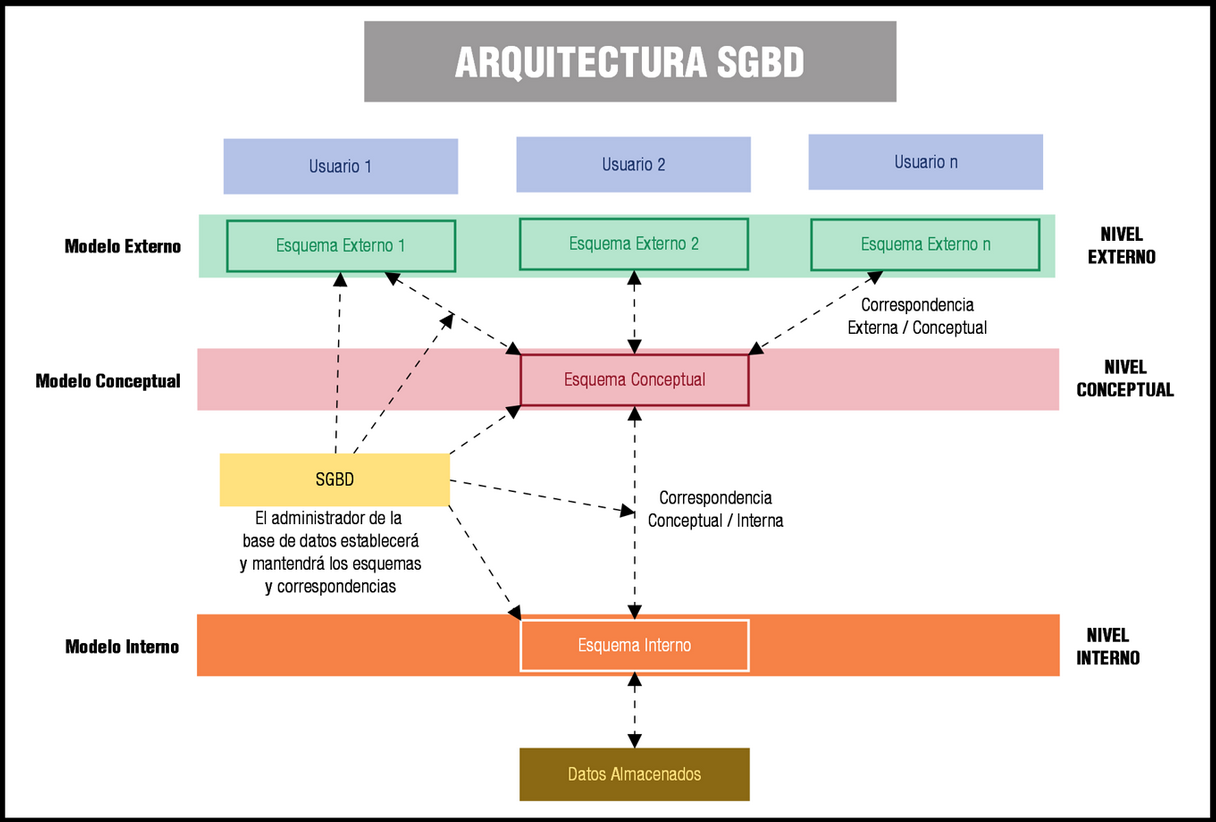
\includegraphics[scale=0.40]{arquitectura-SGBD.png}
    \caption{Arquitectura de SGBD}
\end{figure}

\subsection{Tipos de SGBD}
Una vez que hemos visto las funciones y los componentes de un SGBD, vamos a ver los tipos que podemos encontrarnos atendiendo a diferentes criterios en la siguiente clasificación:

\begin{enumerate}[label=(\alph*)]
    \item \textbf{Modelo Lógico}: este es el primer criterio que nos solemos encontrar. Actualmente, el modelo lógico más empleado es el \textbf{relacional}. Los modelos de red y jerárquicos han quedado obsoletos, pero si hay otros modelos que podemos encontrar como el objeto-relacional. Incluyendo todos los modelos, tenemos:
    \begin{itemize}
        \item Modelo Jerárquico.
        \item Modelo en Red.
        \item Modelo Relacional.
        \item Modelo Orientado a Objetos.
    \end{itemize}

    En la sección 1.4, puede encontrar más información sobre los diferentes modelos y sus características.

    \item \textbf{Número de Usuarios}: también podemos clasificar un SGBD por el número de usuarios al que prestan servicio, pudiendo ser éstos:

    \begin{itemize}
        \item \textbf{Monousuario}: solo atienden a un usuario a la vez y su principal uso en es ordenadores personales.

        \item \textbf{Multiusuario}: atienden a varios usuarios a la vez y entre estos se encuentran la mayoría de SGBD.
    \end{itemize}

    \item \textbf{Distribución de la Base de Datos}: el tercer criterio es el número de sitios en los que esta distribuida la base de datos. Así un SGBD puede ser:

    \begin{itemize}
        \item \textbf{Centralizado}: sus datos se almacenan en un solo computador. Los SGBD centralizados pueden atender a varios usuario, pero la base de datos y el propio sistema de gestión se encuentran alojados en un único computador.

        \item \textbf{Distribuidos} (Homogéneos, Heterogéneos): la base de datos real y el propio SGBD pueden estar distribuidos en varios computadores conectados por red. Dentro de los sistemas distribuidos podemos encontrar dos tipos:

        \begin{itemize}
            \item \textbf{Homogéneos}: utilizan el mismo SGBD en varios computadores diferentes.

            \item \textbf{Heterogéneos}: una tendencia es crear software para acceder a varias bases de datos autónomas preexistentes almacenadas en sistemas distribuidos heterogéneos. Esta da lugar a SGBD federados o \textbf{sistemas multibase de datos}, en los que los SGBD participantes tienen cierto grado de autonomía.
        \end{itemize}
    \end{itemize}

    \item \textbf{Coste del SGBD}: otro criterio de clasificación es el coste del paquete de software, estando en rangos desde los 0 a los 100.000 euros. Mientras que los sistemas más económicos monousuario para microcomputadoras pueden costar entre 0 y 3.000 euros, los paquetes más completos pueden llegar a los 100.000 euros.

    \item \textbf{Propósito}: el último criterio de clasificación es el propósito que tiene el SGBD, es decir, si es de propósito general o específico, siendo estos:

    \begin{itemize}
        \item \textbf{Propósito general}: estos sistemas puede ser utilizado para el tratamiento de cualquier tipo de base de datos.

        \item \textbf{Propósito específico}: cuando el rendimiento es esencial se puede diseñar y construir un software de propósito especial para una aplicación específica, y este sistema solo servirá para esa aplicación. Por ejemplo, muchos sistemas de reserva de líneas aéreas son de propósito especial y pertenecen a la categoría de \textbf{sistemas de procesamiento de transacciones en línea}, que deben atender un gran número de transacciones concurrentes sin imponer excesivos retrasos.
    \end{itemize}
\end{enumerate}

Como vemos, hay muchos tipos de SGBD, ya dependerá de nuestras necesidades y de las restricciones del problema que queremos solventar cual es la elección más adecuada.

\section{SGBD Comerciales}
La elección de un SGBD es una decisión muy importante a la hora de desarrollar proyectos. A veces el sistema más avanzado, el ``mejor'' según los entendidos, puede no ser el más adecuado para el tipo de proyectos que estemos desarrollando. Hemos de tener en cuenta que volumen de carga puede soportar la base de datos, que sistema operativo utilizaremos como soporte, cual es el presupuesto, etc...

Actualmente en el mercado de software existen una gran variedad de SGBD comerciales. En la siguiente figura, mostramos los mas utilizados y cuales son sus características.

\begin{figure}[ht]
    \centering
    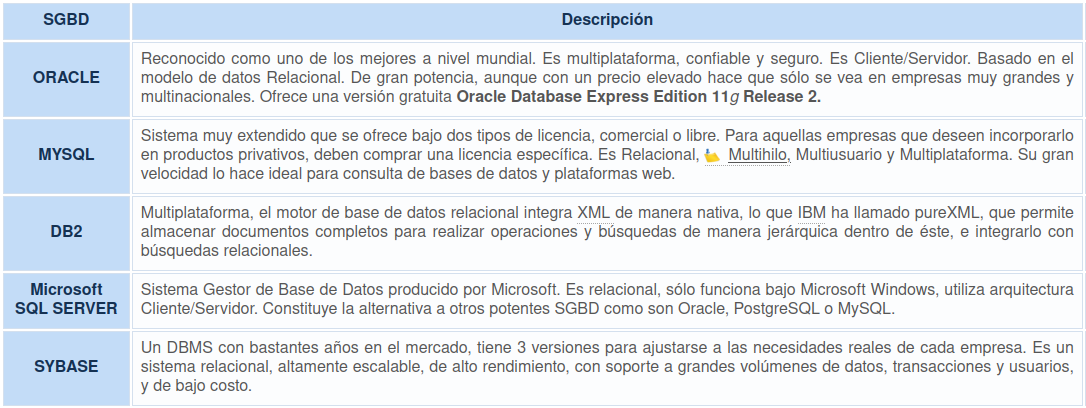
\includegraphics[scale=0.55]{sgdb-comerciales.png}
    \caption{SGBD comerciales}
\end{figure}

Aunque estos son los más importantes, podemos encontrar otros ampliamente usados como DBASE, ACCESS, INTERBASE y FOXPRO.

\section{SGBD Libres}
La alternativa a los SGBD comerciales la tenemos en los SGBD de código abierto o libres, también llamados \textbf{Open Source}. Son sistemas distribuidos y desarrollador libremente. En la siguiente figura se muestran los más importantes así como sus principales características.

\begin{figure}[ht]
    \centering
    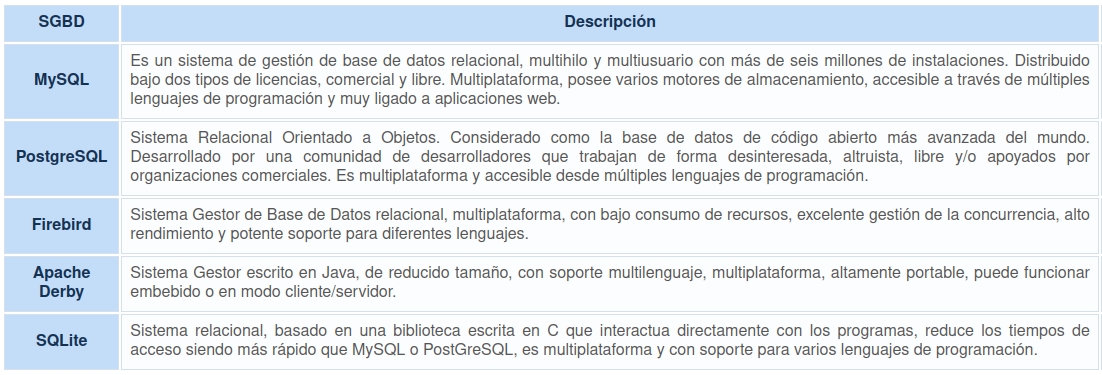
\includegraphics[scale=0.55]{sgdb-libres.png}
    \caption{SGBD libres}
\end{figure}

Cabe también mencionar \textbf{MariaDB}, por la relevancia y uso que esta adquiriendo en aplicaciones web en los últimos años.

\section{Bases de Datos Centralizadas}
Un \textbf{sistema de bases de datos centralizado} es aquel en el que el SGBD esta implantado en una sola plataforma u ordenador desde donde se gestiona directamente, de forma centralizada, la totalidad de los recursos. Es la arquitectura de los centros de procesado de datos tradicionales. Se basa en tecnologías sencillas, muy experimentadas y de gran robustez.

Los sistemas de los años sesenta y setenta era totalmente centralizados, como corresponde a los sistemas operativos de aquellos años, así como al hardware para el que estaban hechos: un gran ordenador para toda la empresa y una red de terminales sin memoria.

Las principales \textbf{características} de los sistemas centralizados son las siguientes:

\begin{itemize}
    \item Se almacena completamente en la ubicación central, es decir, todos los componentes del sistema residen en un único sitio o computador.
    \item No posee múltiples elementos de procesamiento o mecanismos de comunicación como en las bases de datos distribuidas.
    \item Los componentes de la base de datos centralizada son: los datos, el software de gestión de bases de datos y los dispositivos de almacenamiento secundario.
    \item Son sistemas en los que su seguridad puede verse comprometida fácilmente.
\end{itemize}

Estos sistemas, tiene sus ventajas e inconvenientes respecto a los sistemas distribuidos. En la siguiente tabla, puedes ver una lista con los más comunes.

\begin{figure}[ht]
    \centering
    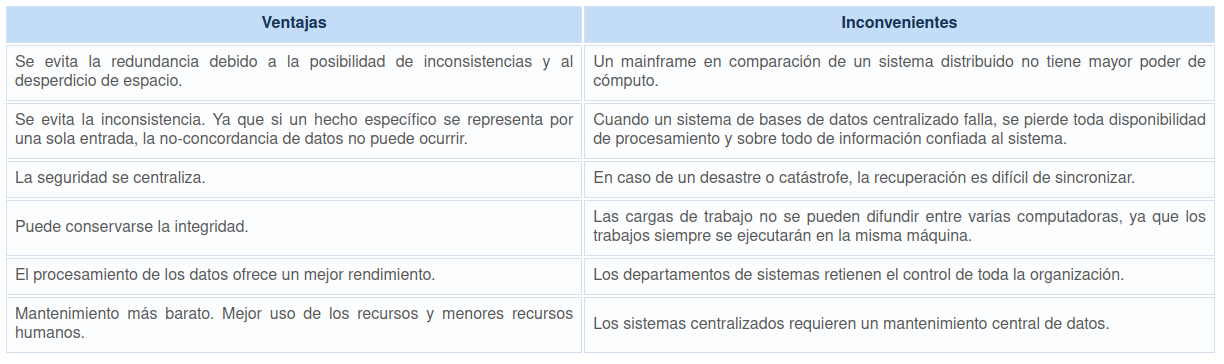
\includegraphics[scale=0.50]{sgbd-central.png}
    \caption{Ventajas e Inconvenientes de las bases de datos centralizadas}
\end{figure}

\section{Bases de Datos Distribuidas}
La necesidad de integrar información de varias de fuentes y la evolución de las tecnologías de la comunicación, han producido cambios muy importantes en los sistemas de bases de datos. La respuesta a estas necesidades y evoluciones se materializa en los sistemas de bases de datos distribuidos.

Dentro de el paradigma de las bases de datos distribuidas, tenemos que tener claras las siguientes definiciones:

\begin{itemize}
    \item \textbf{Base de Datos Distribuida} (\textbf{BDD}): es un conjunto de múltiples bases de datos, lógicamente relacionadas, las cuales se encuentra distribuidas entres diferentes nodos interconectados por una red de comunicaciones.

    \item \textbf{Sistema de Bases de Datos Distribuida} (\textbf{SBDD}): es un sistema en el que múltiples sitios de bases de datos están ligados por un sistema de comunicaciones, de tal forma que, un usuario en cualquier sitio puede acceder a los datos en cualquier parte de la red como si los datos estuvieran almacenados en su propio sitio.

    \item \textbf{Sistema Gestor de Base de Datos Distribuida} (\textbf{SGBDD}): es aquel que se encarga de manejar las BDD y proporciona un mecanismo de acceso que hace que la distribución sea transparente a los usuarios. El termino transparente se refiere a que la aplicación trabajaría, desde un punto de vista lógico, como si un solo SGBD, ejecutado en una sola máquina, administrara esos datos.
\end{itemize}


\begin{figure}[ht]
    \centering
    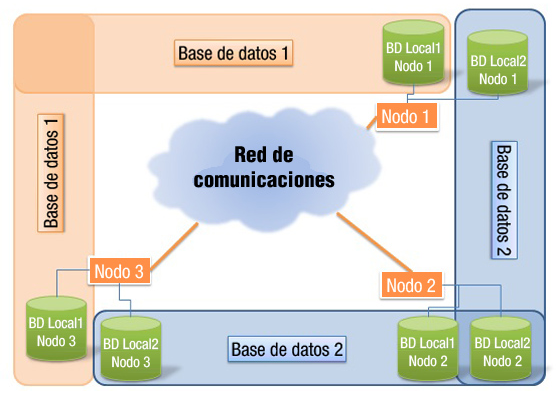
\includegraphics[scale=0.55]{bd-distri.png}
    \caption{Base de datos distribuida}
\end{figure}

Así, un SGBDD desarrollará su trabajo a través de un conjunto de nodos, que poseen un sistema de procesamiento de datos completo con un base de datos local, un sistema gestor de bases de datos e interconectados entre sí. Si estos nodos están dispersos geográficamente, se interconectarán mediante una red de área extensa o WAN (Wide Area Network), pero si se encuentran en edificios relativamente cercanos, puede estar conectados por una red de área local o LAN (Local Area Network).

Este tipo de sistemas es utilizado en organizaciones con estructura descentralizada, industrias de manufactura con múltiples sedes, aplicaciones militares, líneas aéreas, servicios bancarios, etc...

Al igual que las BD centralizadas, las distribuidas tiene sus ventajas e inconvenientes, que podemos ver en la siguiente figura.

\begin{figure}[ht]
    \centering
    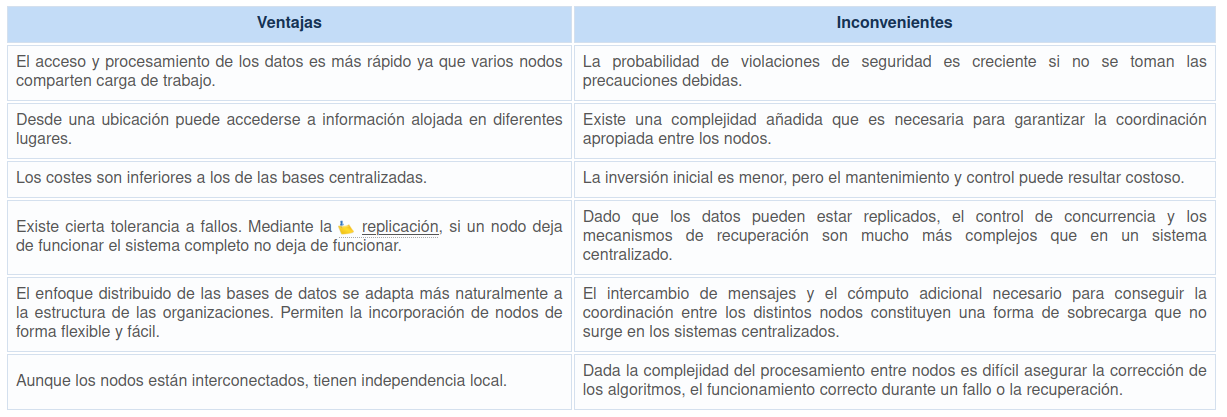
\includegraphics[scale=0.50]{sgbd-distri.png}
    \caption{Ventajas e Inconvenientes de las bases de datos distribuidas}
\end{figure}

\subsection{Fragmentación en Bases de Datos Distribuidas}
Como hemos visto en el punto anterior, la información en las BDD están repartida en diferentes nodos. La forma de extraer los datos consultados se puede hacer mediante la \textbf{fragmentación} de distintas tablas pertenecientes a distintas bases de datos que se encuentran en diferentes servidores. El problema de fragmentación se refiere al particionamiento de la información para distribuir cada parte a los diferentes sitios de la red.

Hay que tener en cuenta el \textbf{grado de fragmentación} que habrá, ya que es un factor clave a la hora de ejecutar las consultas. Si no existe fragmentación, se tomarán las relaciones o tablas como unidad de fragmentación. Pero también puede fragmentarse a nivel de tupla (fila o registro) o a nivel de atributo de una tabla. No será adecuado un grado de fragmentación nulo, ni tampoco un grado de fragmentación demasiado alto. El grado de fragmentación deberá estar equilibrado y responder a las particularidades de las aplicaciones que utilicen dicha base de datos.

Cuando se lleva a cabo la fragmentación, existen \textbf{tres reglas fundamentales} que se deben seguir. A saber:

\begin{itemize}
    \item \textbf{Completitud}: si una relación R se descompone en fragmentos R\textsubscript{1}, R\textsubscript{2}, ..., R\textsubscript{n}, cada elemento de datos que pueda encontrarse en R, deberá encontrarse en uno o varios fragmentos de R\textsubscript{i}.

    \item \textbf{Reconstrucción}: si una relación R se descompone en fragmentos R\textsubscript{1}, R\textsubscript{2}, ..., R\textsubscript{n}, la reconstrucción de la relación a través de sus fragmentos asegura que se preservan las restricciones definidas sobre los datos.

    \item \textbf{Disyunción}: si una relación R se descompone verticalmente, sus atributos primarios clave se repiten en todos sus fragmentos.
\end{itemize}

Así, cada vez que vayamos a diseñar la fragmentación de la información en una BDD, deberemos tener en cuenta estas tres reglas y asegurarnos de que nuestro diseño las cumpla.

Respecto a los \textbf{tipos de fragmentación}, podemos encontrarnos con tres tipos principales:

\begin{itemize}
    \item \textbf{Fragmentación Horizontal}: este tipo de fragmentación se realiza sobre las tuplas de la relación, dividiendo la relación en subrelaciones que contienen un subconjunto de las tuplas que alberga la primera. Dentro de la fragmentación horizontal podemos encontrar la \textbf{primaria} y la \textbf{secundaria}.

    \item \textbf{Fragmentación Vertical}: la fragmentación vertical se basa en los atributos de la relación para efectuar la división. Una relación R produce fragmentos  R\textsubscript{1}, R\textsubscript{2}, ..., R\textsubscript{n}, cada uno de los cuales contiene un subconjunto de atributos de R así como la clave primaria de R. El objetivo de la fragmentación es particionar una relación en un conjunto de relaciones mas pequeñas de forma que varias aplicaciones de usuario se ejecutarán sobre un fragmento. En este contexto, una fragmentación óptima es aquella que produce un esquema de fragmentación que minimiza el tiempo de ejecución de las consultas de usuario. La fragmentación vertical es más complicada que la horizontal, ya que existe un número mayor de alternativas para realizarla.

    \item \textbf{Fragmentación Híbrida o Mixta}: podemos combinar ambas aproximaciones utilizando la denominada fragmentación mixta. Si tras una fragmentación horizontal se lleva a cabo una vertical, se habla de fragmentación mixta Horizontal-Vertical. Para el caso contrario, estaremos ante una fragmentación Vertical-Horizontal. Estos dos tipos de fragmentación se representan mediante arboles.
\end{itemize}

\section{Enlaces de Ampliación}
 En este tema hemos visto los conceptos básicos sobre el almacenamiento de la información, centrándonos en los conceptos de ficheros y sus características, en que es una base de datos y las diferentes modelos de organización que se suelen emplear, viendo por último en que consiste un sistema gestos de bases de datos y que tipos existen.

 A continuación, mostramos una lista con enlaces para ampliar y profundizar más en esta información, principalmente en los aspectos relacionados con las bases de datos y los SGBD.

 \begin{itemize}
     \item SGBD MariaDB
     \\\url{https://es.wikipedia.org/wiki/MariaDB}

     \item SGBD MongoDB
     \\\url{https://es.wikipedia.org/wiki/MongoDB}

     \item SGBD PostgreSQL
     \\\url{https://es.wikipedia.org/wiki/PostgreSQL}

     \item Formato JSON para el intercambio de datos
     \\\url{https://es.wikipedia.org/wiki/JSON}

     \item Formato BSON para el intercambio de datos
     \\\url{https://es.wikipedia.org/wiki/BSON}

     \item Información sobre sistemas de gestión tipo NoSQL
     \\\url{https://es.wikipedia.org/wiki/NoSQL}
 \end{itemize}

Además de estos enlaces, podemos encontrar muchísima más información sobre los diferentes SGBD en sus correspondientes páginas oficiales, que podemos encontrar con una búsqueda rápida en cualquier buscador web, ya que la mayoría contienen una extensa documentación.

\chapter{Unidad 2: Bases de Datos Relacionales - TODO}
\chapter{Unidad 3: Implantación de Bases de Datos Relacionales - TODO}

\chapter{Unidad 4: Realización de Consultas}
En esta unidad vamos a ver como realizar consultas a una base de datos usando \textbf{SQL}. Usaremos como bases de datos para realizar la consultas \textbf{MySQL} y \textbf{Oracle}, por ello hay que tener en cuenta que, aunque hay \textbf{aspectos comunes} de SQL a ambos sistemas de gestión de bases de datos, también hay aspectos específicos, en cuyo caso se indicará explícitamente.

\section{Introducción}

El lenguaje \textbf{SQL} nació a partir de la publicación ``A realational model of data for large shared banks'', publicado por \textbf{Edgar Frank Codd}. IBM aprovecho el modelo propuesto por Codd para crear un lenguaje acorde al recién creado \textbf{modelo relacional}, llamándolo \textbf{SEQUEL} (Structured English Query Language). Con el tiempo, SEQUEL se convertiría en SQL (Structured Query Language). En 1979, la empresa \textbf{Relational Software} lanzaría la primera versión comercial de SQL. Esta empresa, la conocemos hoy en día como \textbf{Oracle}.

En 1992, \textbf{ANSI} e \textbf{ISO} completaron la estandarización de SQL y se definieron las sentencias básicas que debía contener SQL para que fuera estándar. A este se le conocería como ANSI-SQL o SQL92.

Hoy en día, SQL sigue siendo el lenguaje estándar de acceso a bases de datos relacionales. La mayoría de bases de datos cumplen con el estándar, aunque cada fabricante añade sus mejoras al lenguaje SQL.

La \textbf{primera fase de trabajo} con cualquier base de datos consiste en al utilización de un lenguaje \textbf{DDL} (Data Defining Language), que nos permitirá crear la bases de datos y sus tablas, algo necesario antes de comenzar a trabajar con los datos que queremos alojar en esta. Esta fase la desarrollamos en la unidad anterior.

La \textbf{siguiente fase} será manipular los datos, trabajando con sentencias \textbf{DML} (Data Management Language). Este lenguaje esta orientado a consultas y manejo de datos de los datos creados. Las principales sentencias que nos proporciona son \textbf{SELECT}, \textbf{INSERT}, \textbf{DELETE} y \textbf{UPDATE}.

En esta unidad nos centraremos en las consultas, es decir, en la sentencia \textbf{SELECT}.

\subsection{En Oracle}
Las sentencias que veremos a continuación pueden ser ejecutadas desde el entorno web \textbf{Application Express} de Oracle utilizando el botón \textbf{SQL Workshop} en la página de inicio o home y eligiendo la opción \textbf{SQL Commands}.

También se pueden indicar las sentencias desde el entorno \textbf{SQL*PLus} que ofrece Oracle y que puede encontrarse  en \textbf{Inicio > Todos los Programas > Oracle Database 11g Express Edition > Run SQL Command Line}, en el menú inicio de Windows.

Si optas por usar esta última aplicación, el primera paso que debes realizar para poder manipular los datos de una determinada tabla, es conectarse utilizando un nombre de usuario con los permisos necesarios para acceder a ese tipo de operaciones en la tabla deseada. Utiliza para ello la orden \textbf{CONNECT} seguida del nombre de usuario. Posteriormente solicitará la contraseña de usuario correspondiente.

Para ejecutar cualquier de las sentencias SQL que aprenderás en los siguiente puntos, simplemente debes\textbf{ escribirla completa} y pulsar \textbf{Intro} para que se inicie su ejecución.

\subsection{MySQL}
En el caso de \textbf{MySQL}, las sentencias que veremos a continuación pueden ser ejecutadas:

\begin{itemize}
    \item Desde cualquier \textbf{cliente gráfico} como por ejemplo \textbf{MySQL Workbench}. En este caso, redactaremos la sentencia en la ventana \textbf{SQL} y la ejecutaremos accediendo a \textbf{Query > Execute Current Statement}, o mediante el botón con un símbolo de un \textbf{rayo amarillo}.
    \item Desde la \textbf{línea de comandos} de MySQL.
\end{itemize}

En ambos casos, lo primero que habrá que hacer es iniciar o arrancar el servidor de bases de datos MySQL, si no esta iniciado por defecto, y conectar o abrir una conexión con el servidor utilizando un nombre de usuario con los permisos necesarios para hacer este tipo de operaciones sobre la bases de datos en la que queremos trabajar.

\subsection{Modelo de la Base de Datos de Ejemplo}
Aquí vamos a exponer los diferentes diagramas de la base de datos que vamos a usar como ejemplo en este tema, tanto para Oracle como para MySQL.

\begin{itemize}
    \item \textbf{Modelo para Oracle}: en primero lugar vamos a mostrar el esquema entidad-relación de la base de datos con la que vamos a trabajar en Oracle.

    \begin{figure}[H]
        \centering
        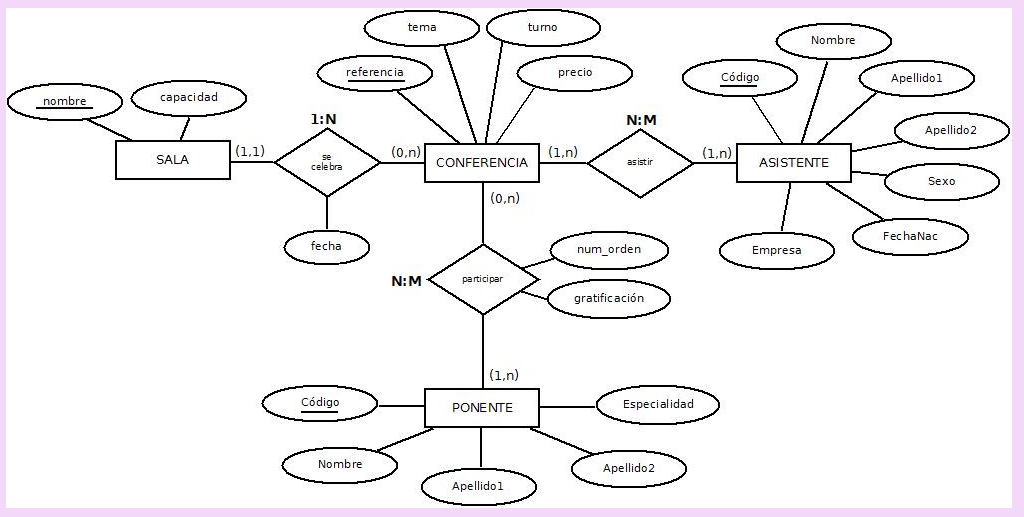
\includegraphics[scale=0.45]{esquema-entidad-relacion.png}
        \caption{Esquema entidad relación para la base de datos Oracle}
    \end{figure}

    El \textbf{modelo relacional} de paso de tablas resultante del anterior esquema sería el siguiente:

    \begin{figure}[H]
        \centering
        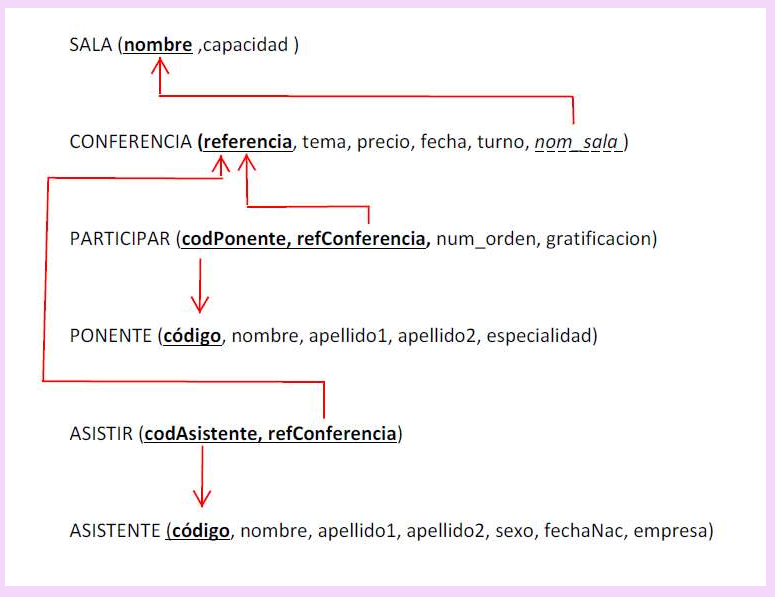
\includegraphics[scale=0.35]{esquema-paso-tablas.png}
        \caption{Esquema de paso a tablas para Oracle}
    \end{figure}

    \item \textbf{Modelo para MySQL}: para MySQL vamos a emplear otra base de datos. En primer lugar, aquí tenemos el \textbf{grafo relacional} para el paso de tablas, en modo texto, de esta base de datos.

    \begin{figure}[H]
        \centering
        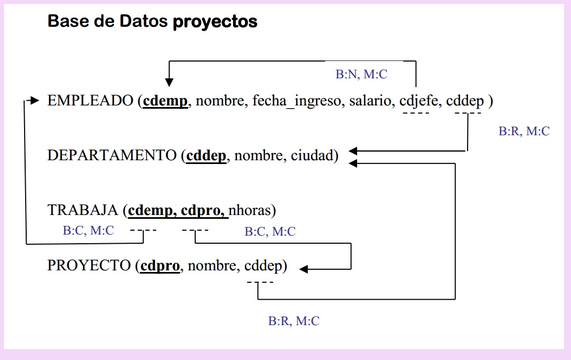
\includegraphics[scale=0.55]{grafo-relacional-mysql.png}
        \caption{Grafo relacional de la base de datos para MySQL}
    \end{figure}

    A partir de este modelo, se ha creado uno dentro de la aplicación \textbf{WorkBench}, el cual podemos ver en la siguiente imagen:

    \begin{figure}[H]
        \centering
        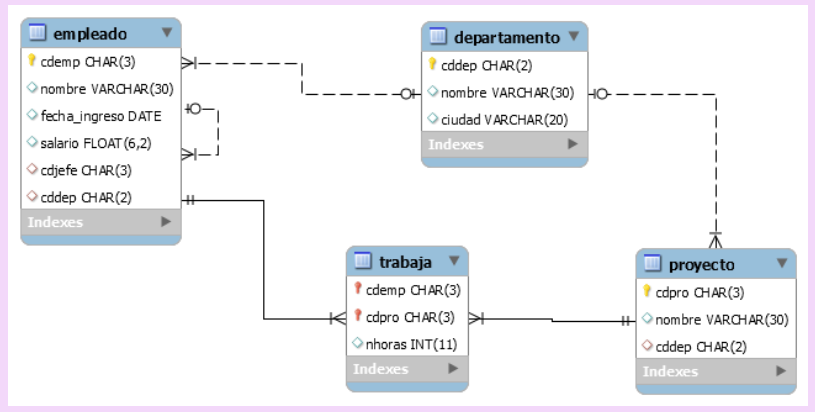
\includegraphics[scale=0.40]{esquema-workbench.png}
        \caption{Esquema relacional en Workbench para MySQL}
    \end{figure}
\end{itemize}

Además os recomendamos que consultéis el apéndice \textbf{Anexos Tema 4} donde se explica más detalladamente como crear las bases de datos, tanto en Oracle como MySQL, que vamos a emplear en esta unidad.

\section{La Sentencia SELECT}
En esta unidad, como hemos comentado, vamos a estudiar la realización de \textbf{consultas} a una bases de datos. El lenguaje SQL nos proporciona la sentencia \textbf{SELECT} para realizar dichas consultas, permitiéndonos recuperar o seleccionar datos de una o varias tablas.

Esta sentencia consta de 4 partes básicas:

\begin{itemize}
    \item \textbf{Cláusula SELECT}, seguida de la descripción de lo que se desea ver, es decir, de los \textbf{nombres de la columnas} que quieres que se muestren, separados por comas simples. Esta parte es \textbf{obligatoria}.

    \item \textbf{Cláusula FROM}, seguida del \textbf{nombre} de la \textbf{tabla o tablas} de las que queremos consultar las columnas, es decir, de donde quieres extraer los datos. Esta parte también es \textbf{obligatoria}.

    \item \textbf{Cláusula WHERE}, seguida de un \textbf{criterio de selección} o \textbf{condición}. Esta parte es \textbf{opcional}.

    \item \textbf{Cláusula ORDER BY}, seguida por un criterio de ordenación. Esta cláusula también es \textbf{opcional}.
\end{itemize}

Por lo tanto, una sentencia SELECT completa quedaría de la siguiente forma:

\begin{figure}[h]
    \begin{tcolorbox}[sharp corners, colback=yellow!30, colframe=white!20]
        \tiny
        \begin{verbatim}

 SELECT [ALL | DISTINCT] columna1, columna2, ... FROM tabla1, tabla2, ... WHERE condición1, ... ORDER BY ordenación;
        \end{verbatim}
    \end{tcolorbox}
\end{figure}

Las cláusulas \textbf{ALL} y \textbf{DISTINC} son opcionales, y su funcionalidad es la siguiente:

\begin{itemize}
    \item \textbf{ALL}: esta cláusula indica que se quieren seleccionar todas las filas, \textbf{estén o no repetidas}. Es el \textbf{valor por defecto} y no se suele especificar.

    \item \textbf{DISTINC}: esta cláusula indica que las filas repetidas se deben suprimir del resultado.
\end{itemize}

En los siguientes puntos, veremos más a fondo cada una de las cláusulas que acabamos de ver.

\subsection{Cláusula SELECT}
Esta cláusula es la principal de la sentencian \textbf{SELECT}, que nos permitirá seleccionar la información que queremos obtener. Además de ser obligatoria, debemos tener en cuenta lo siguiente:

\begin{itemize}
    \item \textbf{Se pueden nombrar} a las columnas anteponiendo el nombre de la tabla de la que proceden, aunque esto es opcional, el resultado sería así: \textbf{nombretabla.nombrecolumna}.

    \item Si queremos \textbf{incluir todas las columnas} podemos usar el comodín \textbf{asterisco} (*). Por ejemplo: \textbf{SELECT * FROM nombretabla}.

    \item También podemos \textbf{ponerle alias a los nombres} de las columnas. Cuando se consulta una base de datos, los nombres de las columnas se usan como cabeceras de presentación. Si este resulta largo, corto o poco descriptivo, podemos usar un alias. Para ello, ponemos a continuación del nombre de la columna, el alias que le demos a esta entre comillas. Por ejemplo:

    \begin{itemize}
        \item \textbf{Oracle}:

        \begin{figure}[H]
            \begin{tcolorbox}[sharp corners, colback=yellow!30, colframe=white!20]
                \scriptsize
                \begin{verbatim}


                     SELECT nombre "Nombre de la Sala" FROM SALA;
                \end{verbatim}
            \end{tcolorbox}
        \end{figure}

         \item \textbf{MySQL}:

         \begin{figure}[H]
         \begin{tcolorbox}[sharp corners, colback=yellow!30, colframe=white!20]
             \scriptsize
             \begin{verbatim}


                     SELECT nombre "Nombre de la Sala" FROM SALA;

                     SELECT nombre as "Nombre empleado" FROM empleado;
             \end{verbatim}
         \end{tcolorbox}
         \end{figure}
    \end{itemize}

    \item También podemos \textbf{sustituir} el nombre de las columnas por \textbf{\gls{constantes}}, \textbf{\gls{expresiones}} o \textbf{\gls{funciones}} SQL, como vemos en los siguientes ejemplos.

    \begin{itemize}
        \item \textbf{Oracle}:

        \begin{figure}[h]
            \begin{tcolorbox}[sharp corners, colback=yellow!30, colframe=white!20]
                \scriptsize
                \begin{verbatim}


                     SELECT 4*3/100 "MiExpresión",capacidad FROM SALA;
                \end{verbatim}
            \end{tcolorbox}
        \end{figure}

        \item \textbf{MySQL}:

         \begin{figure}[h]
            \begin{tcolorbox}[sharp corners, colback=yellow!30, colframe=white!20]
                \scriptsize
                \begin{verbatim}


                    SELECT 4*3/100 "MiExpresión", nombre FROM empleado;
                \end{verbatim}
            \end{tcolorbox}
        \end{figure}
    \end{itemize}
\end{itemize}

\subsection{Cláusula FROM}
Al realizar una sentencia SELECT debemos especificar de donde vamos a extraer los datos, es decir, de que tablas vamos a recuperar la información, para ello disponemos de la cláusula \textbf{FROM}.

En esta cláusula es donde se \textbf{definen} los \textbf{nombres de las tablas}. Si aparecen más de un tabla, éstas irán separadas por comas.  A este tipo de consulta se denomina \textbf{consulta combinada} o \textbf{join}. Más adelante veremos que para que este tipo de consultas puedan realizarse deberemos aplicar una condición de combinación a través de la clausula \textbf{WHERE}.

En el caso de \textbf{Oracle}, también puedes añadir el nombre de usuario del \textbf{propietario} de estas tablas, indicándolo así \textbf{USUARIO.TABLA}, pudiendo así distinguir entre tablas de un usuario y otro.

Tanto en \textbf{Oracle} como en \textbf{MySQL} pueden utilizarse un alias en las tablas para abreviar, en este casi, \textbf{no es necesario} encerrar el alias \textbf{entre comillas}, como en el caso de SELECT.

\begin{itemize}
    \item \textbf{Oracle}:

     \begin{figure}[H]
     \begin{tcolorbox}[sharp corners, colback=yellow!30, colframe=white!20]
         \scriptsize
         \begin{verbatim}


                            SELECT * FROM CONFERENCIA C;
         \end{verbatim}
     \end{tcolorbox}
     \end{figure}

     \item \textbf{MySQL}:

     \begin{figure}[H]
     \begin{tcolorbox}[sharp corners, colback=yellow!30, colframe=white!20]
         \scriptsize
         \begin{verbatim}


                             SELECT * FROM empleado e;
         \end{verbatim}
     \end{tcolorbox}
     \end{figure}
\end{itemize}

\subsection{Cláusula WHERE}
Hasta ahora hemos podido usar la sentencia SELECT para obtener todas o un subconjunto de columnas de una o varias tablas, pero esta selección afectaba a todas las filas de la tabla. Si queremos restringir esta selección a un subconjunto de filas, debemos especificar alguna condición que deban cumplir aquellos registros que queremos seleccionar. Para esto, debemos emplear la cláusula \textbf{WHERE}.

A continuación de la palabra \textbf{WHERE} será donde pongamos la condición que han de cumplir las filas para salir  como resultados de dicha consulta.

El criterio de búsqueda o condición puede ser más o menos sencillo y para crearlo se pueden combinar operadores de diversos tipos, funciones o expresiones más o menos complejas.

\begin{itemize}
    \item \textbf{Oracle}:

    \begin{figure}[H]
        \begin{tcolorbox}[sharp corners, colback=yellow!30, colframe=white!20]
            \scriptsize
            \begin{verbatim}


          SELECT nombre, apellido1, apellido2 FROM ASISTENTE WHERE sexo = 'H';
            \end{verbatim}
        \end{tcolorbox}
    \end{figure}

    \item \textbf{MySQL}:

    \begin{figure}[H]
        \begin{tcolorbox}[sharp corners, colback=yellow!30, colframe=white!20]
            \scriptsize
            \begin{verbatim}


                SELECT nombre FROM empleado WHERE salario < 2000;
            \end{verbatim}
        \end{tcolorbox}
    \end{figure}
\end{itemize}

\subsection{Cláusula HAVING}
En el apartado anterior veíamos las funciones de \textbf{WHERE}, el problema es que si en la condición queremos incluir operadores aritméticos, como \textbf{SUM}, \textbf{MAX}, \textbf{COUNT}.., ya no sería posible utilizarlo. Aquí es cuando viene en nuestra ayuda \textbf{HAVING}.

Si cuando hacemos una consulta queremos restringir la selección a un subconjunto de filas especificando una condición aritmética debemos usar la clausula \textbf{HAVING}.

Por lo tanto, si queremos saber cuando debemos usar \textbf{HAVING} o \textbf{WHERE} debemos tener en cuenta esta condición, ademas de que \textbf{WHERE} se usa para operar sobre \textbf{registros individuales} mientras \textbf{HAVING} se usa para operar sobre conjuntos de registros.

\begin{itemize}
    \item \textbf{Oracle}: si en nuestra tabla \textbf{ASISTENTE}, necesitáramos un listado de los asistentes a más de dos películas, bastaría con crear la siguiente consulta.

    \begin{figure}[H]
        \begin{tcolorbox}[sharp corners, colback=yellow!30, colframe=white!20]
            \scriptsize
            \begin{verbatim}


                SELECT nombre, apellido1, apellido2
                FROM ASISTENTE
                GROUP BY nombre
                HAVING count(peliculas) > 2;
            \end{verbatim}
        \end{tcolorbox}
    \end{figure}

    \item \textbf{MySQL}: si en nuestra tabla \textbf{empleado}, necesitáramos un listado de los empleados con un salario inferior a 200€, bastaría con crear la siguiente consultar:

    \begin{figure}[H]
        \begin{tcolorbox}[sharp corners, colback=yellow!30, colframe=white!20]
            \scriptsize
            \begin{verbatim}


                SELECT nombre
                FROM empleado
                GROUP BY nombre
                HAVING AVG(salario) < 200;
            \end{verbatim}
        \end{tcolorbox}
    \end{figure}
\end{itemize}

Normalmente \textbf{HAVING} suele ir acompañado de \textbf{GROUP BY}, ya que éste opera sobre los grupos que devuelve la la sentencia \textbf{GROUP BY}.

\subsection{Cláusula ORDE BY}
En la consulta del punto anterior hemos obtenido una lista de nombres y apellidos de los empleados. Sería conveniente que quedara ordenador por apellidos ya que es más práctico. Para ello, vamos a usar la cláusula \textbf{ORDER BY}.

Con esta cláusula, podemos \textbf{ordenar} la respuesta que recibimos a nuestra consulta especificando un \textbf{criterio de ordenación}. Su sintaxis sería la siguiente:

\begin{tcolorbox}[sharp corners, colback=yellow!30, colframe=white!20]
    \scriptsize
    \begin{verbatim}


      SELECT [ALL | DISTINCT] columna1, columna2, ...
      FROM tabla1, tabla2, ...
      WHERE condición1, condición2, ...
      ORDER BY columna1 [ASC | DESC], columna2 [ASC | DESC], …, columnaN [ASC | DESC];
    \end{verbatim}
\end{tcolorbox}

Después de cada columna de ordenación se puede incluir el \textbf{tipo de ordenación} (ascendente o descendente) utilizando las palabras reservadas \textbf{ASC} o \textbf{DESC}. Por defecto, la ordenación es de tipo ascendente.

Debes saber que es posible \textbf{ordenar} por \textbf{mas de una columna}. Es más, puedes ordenar no solo por columnas sino a través de una expresión creada con columnas, una constante o funciones SQL.

También se puede referenciar el campo por su número de orden en lugar de su nombre, es decir, referenciarlo por su posición en la lista de selección.

\begin{itemize}
    \item \textbf{Oracle}:

    \begin{figure}[H]
        \begin{tcolorbox}[sharp corners, colback=yellow!30, colframe=white!20]
            \scriptsize
            \begin{verbatim}


        SELECT nombre, apellido1, apellido2,
        FROM ASISTENTE
        ORDER BY apellido1, apellido2, nombre;

        -- O bien seleccionandolo por el número de campo

        SELECT nombre, apellido1, apellido2, empresa FROM ASISTENTE ORDER BY 4;
            \end{verbatim}
        \end{tcolorbox}
    \end{figure}

    \item \textbf{MySQL}:

    \begin{figure}[H]
        \begin{tcolorbox}[sharp corners, colback=yellow!30, colframe=white!20]
            \scriptsize
            \begin{verbatim}

               SELECT nombre, cddep FROM empleado ORDER BY cddep, nombre;S

               SELECT nombre, cddep, salario FROM empleado ORDER BY 3;
            \end{verbatim}
        \end{tcolorbox}
    \end{figure}
\end{itemize}

Hay que tener en cuenta que si colocamos un \textbf{número mayor que la cantidad de campos} de la lista de selección, aparecerá un \textbf{mensaje de error} y la consulta no se ejecutará. Además, no todos los \textbf{tipos de datos}  sirven para ordenar, solo servirán aquellos de tipo \textbf{carácter}, \textbf{número} y \textbf{fecha}.

\subsection{Tipos de JOIN}
La palabra \textbf{JOIN} significa unir, y precisamente ese es su uso en SQL. Esta sentencia se usa para \textbf{combinar filas} de distintas tablas con campos comunes entre ellas. Hay diferentes tipos de \textbf{JOIN}, los cuales podemos ver en la siguiente figura.

\begin{figure}[H]
    \centering
    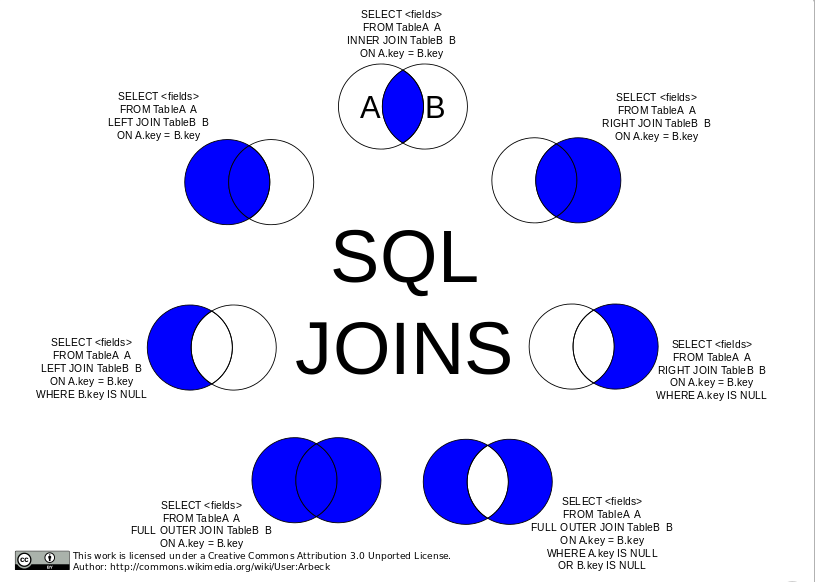
\includegraphics[scale=0.40]{tipos-join.png}
    \caption{Tipos de JOIN}
\end{figure}

A continuación vamos a explicar un poco cada tipo y a poner un ejemplo de cada uno de ellos.

\begin{itemize}
    \item \textbf{INNER JOIN}: devuelve como resultado la selección de las distintas filas que tengan columnas en ambas tablas. Por ejemplo, si tenemos dos tablas, Empleados y Departamentos, y queremos listar los departamentos al cual pertenece cada empleado, la sentencia sería la siguiente:

    \begin{figure}[H]
        \begin{tcolorbox}[sharp corners, colback=yellow!30, colframe=white!20]
            \scriptsize
            \begin{verbatim}


                SELECT de.nombre, e.nombre
                FROM departamento de
                INNER JOIN empleados e
                ON de.id = e.departamento;
            \end{verbatim}
        \end{tcolorbox}
    \end{figure}

    \item \textbf{RIGHT JOIN}: devuelve como resultado todas las filas de la tabla de la derecha más las coincidencias con la tabla de la izquierda. Por ejemplo, si tenemos dos tablas, Empleados y Proyectos, vamos a listar los empleados que están asignados a algún proyecto.

    \begin{figure}[H]
        \begin{tcolorbox}[sharp corners, colback=yellow!30, colframe=white!20]
            \scriptsize
            \begin{verbatim}


SELECT p.nombre, e.nombre FROM proyectos p RIGHT JOIN empleados e  ON p.id = e.proyecto;
            \end{verbatim}
        \end{tcolorbox}
    \end{figure}

    \item \textbf{LEFT JOIN}: devuelve como resultado todas las filas de la tabla izquierda más las coincidencias con la tabla de la derecha. Por ejemplo, si tenemos dos tablas Empleados y Proyectos, vamos a listar los empleados y aparecerán los proyectos que están asignados a algún empleado:

    \begin{figure}[H]
        \begin{tcolorbox}[sharp corners, colback=yellow!30, colframe=white!20]
            \scriptsize
            \begin{verbatim}


SELECT p.nombre, e.nombre FROM proyectos p LEFT JOIN empleados e  ON p.id = e.proyecto;
            \end{verbatim}
        \end{tcolorbox}
    \end{figure}

    \item \textbf{OUTER JOIN} o \textbf{FULL OUTER JOIN}: devuelve como resultado todas las filas de la tabla de la derecha y todas las filas de la tabla de la izquierda. Aparecerá \textbf{NULL} cuando no haya una coincidencia. Por ejemplo, si tenemos dos tablas Empleados y Proyectos, vamos a listar todos los proyectos y todos los empleados:

    \begin{figure}[H]
        \begin{tcolorbox}[sharp corners, colback=yellow!30, colframe=white!20]
            \scriptsize
            \begin{verbatim}


SELECT p.nombre, e.nombre FROM proyectos p OUTER JOIN empleados e ON p.id = e.proyecto;
            \end{verbatim}
        \end{tcolorbox}
    \end{figure}

    La opción \textbf{OUTER JOIN} no existe en \textbf{MySQL}, por lo que cuando queramos usar una sentencia similar deberemos usar la cláusula \textbf{UNION}, entre dos consultas de tipo \textbf{LEFT JOIN} y \textbf{RIGHT JOIN}, como se muestra a continuación.

    \begin{figure}[H]
        \begin{tcolorbox}[sharp corners, colback=yellow!30, colframe=white!20]
            \scriptsize
            \begin{verbatim}


SELECT p.nombre, e.nombre FROM proyectos p LEFT JOIN empleados e  ON p.id = e.proyecto

UNION

SELECT p.nombre, e.nombre FROM proyectos p RIGHT JOIN empleados e  ON p.id = e.proyecto;
            \end{verbatim}
        \end{tcolorbox}
    \end{figure}
\end{itemize}

\section{Operadores}
Como hemos visto en el punto anterior, con la cláusula \textbf{WHERE} podíamos incluir expresiones para filtrar el conjunto de datos que queríamos consultar. Para crear estas expresiones, necesitamos usar diferentes operadores de modo que se puedan comparar, utilizar la lógica o elegir en función de la suma, etc...

Los \textbf{operadores} son símbolos que permiten la realización de operaciones matemáticas, lógicas, concatenar cadenas.., entre otras cosas. \textbf{Oracle} reconoce 4 tipos diferentes de operadores. A saber:

\begin{enumerate}
    \item \textbf{Relacionales} o de \textbf{comparación}.
    \item \textbf{Aritméticos}.
    \item De \textbf{concatenación}.
    \item \textbf{Lógicos}.
\end{enumerate}

En los siguientes apartados vamos a ver cuales son cada uno de los operadores dentro de estas categorías, para que sirven y como se usan.

\subsection{Operadores Relacionales}
Los \textbf{operadores relacionales} nos permitirán \textbf{comparar expresiones}, que pueden ser valores concretos de campo, variables, etc...

Son símbolos que se usan para comparar dos valores. Si el \textbf{resultado} de la comparación es \textbf{correcto}, la \textbf{expresión} considerada es \textbf{verdadera}, en \textbf{caso contrario}, es \textbf{falsa}.

En la siguiente figura, puedes ver una tabla con todos los operadores relacionales que podemos usar en SQl y su significado.

\begin{figure}[H]
    \centering
    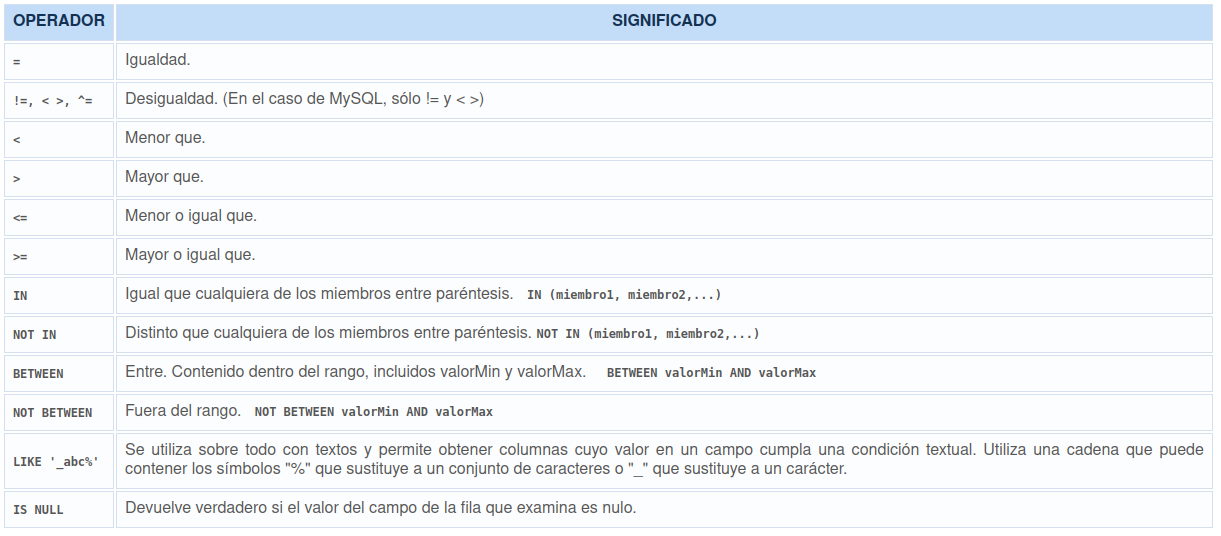
\includegraphics[scale=0.50]{operadores-relacionales.png}
    \caption{Tabla de operadores relacionales}
\end{figure}

El \textbf{valor NULL} significa valor inexistente o desconocido y por tanto es tratado de forma diferente al resto de valores. Si queremos verificar que un valor es \textbf{NULL} los operadores que acabamos de ver no serán válidos. Deberemos usar el operador \textbf{IS NULL} o \textbf{IS NOT NULL} como se indica en la tabla, que nos devolverá verdadero si el valor es NULL o no respectivamente.

Además, cuando se usa \textbf{ORDER BY}, los valores se NULL se muestran en primer lugar si se usa el modo ascendente o el último si se usa el descendente.

A continuación, vemos dos ejemplo del uso de operadores tanto en Oracle como MySQL.

\begin{itemize}
    \item \textbf{Oracle}: si queremos obtener el nombre completo de los ponentes cuyo código comienza por ESP ordenados alfabéticamente por el primer apellido seria:

    \begin{figure}[h]
        \begin{tcolorbox}[sharp corners, colback=yellow!30, colframe=white!20]
            \scriptsize
            \begin{verbatim}


  SELECT nombre, apellido1, apellido2 FROM PONENTE WHERE codigo LIKE
  'ESP%' ORDER BY apellido1;
            \end{verbatim}
        \end{tcolorbox}
    \end{figure}

    \item \textbf{MySQL}: si queremos obtener aquellos empleados cuyo salario es superior a 1000€ podemos crear la siguiente consulta:

    \begin{figure}[H]
        \begin{tcolorbox}[sharp corners, colback=yellow!30, colframe=white!20]
            \scriptsize
            \begin{verbatim}


         SELECT nombre, salario FROM empleado WHERE salario > 1000;
            \end{verbatim}
        \end{tcolorbox}
    \end{figure}
\end{itemize}

\subsection{Operadores Aritméticos}
Los \textbf{operadores aritméticos} son aquellos que nos permiten realizar cálculos matemáticos con valores numéricos. Con estos operadores, \textbf{es posible obtener} salidas en la cuales \textbf{una columna} sea el \textbf{resultado de un cálculo} y no un campo de una tabla

En la siguiente tabla vemos los principales operadores aritméticos.

\begin{figure}[H]
    \centering
    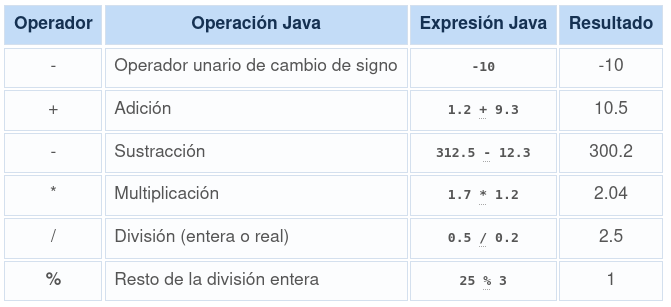
\includegraphics[scale=1]{operadores-aritmeticos.png}
    \caption{Operadores aritméticos en SQL}
\end{figure}

Ejemplo de usos de operadores aritméticos son los siguientes:

\begin{itemize}
    \item \textbf{Oracle}: si queremos obtener el precio de una conferencia aumentado en un 5\% en aquellas conferencia inferiores a 15€, podemos realizar la siguiente consulta:

    \begin{figure}[h]
        \begin{tcolorbox}[sharp corners, colback=yellow!30, colframe=white!20]
            \scriptsize
            \begin{verbatim}


                SELECT precio*1,05 FROM CONFERENCIA WHERE precio<15;
            \end{verbatim}
        \end{tcolorbox}
    \end{figure}

    \item \textbf{MySQL}: si queremos obtener el salario aumentado un 5\% de aquellos trabajadores que cobran menos de 2000€, la consulta será la siguiente:

    \begin{figure}[h]
        \begin{tcolorbox}[sharp corners, colback=yellow!30, colframe=white!20]
            \scriptsize
            \begin{verbatim}


                SELECT salario*1.05 FROM empleado WHERE salario<=2000;
            \end{verbatim}
        \end{tcolorbox}
    \end{figure}
\end{itemize}

Hay que tener en cuenta que que cuando una expresión se calcula sobre un valor \textbf{NULL} el resultado es el propio valor \textbf{NULL}.

Además de estos operadores, en \textbf{Oracle} tenemos el operador '\textbf{||}', que nos permite \textbf{concatenar cadenas de caracteres}. Oracle puede, además, convertir automáticamente valores numéricos en cadenas de caracteres para una concatenación. En \textbf{MySQL}, en cambio, se usa la función \textbf{CONCAT(cadena1, cadena2,..)} para la concatenación de cadenas.

\begin{itemize}
    \item \textbf{Oracle}: si queremos mostrar juntos el primer y segundo apellido de un ponente, podemos usar la siguiente consulta:

    \begin{figure}[h]
        \begin{tcolorbox}[sharp corners, colback=yellow!30, colframe=white!20]
            \scriptsize
            \begin{verbatim}


                SELECT nombre, apellido1 || apellido2 FROM PONENTE;


                -- Si queremos dejar un espacio entre una apellido y otro...


                SELECT nombre, apellido2 || " " || apellido2 FROM PONENTE;
            \end{verbatim}
        \end{tcolorbox}
    \end{figure}

    \item \textbf{MySQL}: para obtener en una sola columna el nombre y el código de empleado, utilizamos la función CONCAT de la siguiente manera:

    \begin{figure}[h]
        \begin{tcolorbox}[sharp corners, colback=yellow!30, colframe=white!20]
            \scriptsize
            \begin{verbatim}


                SELECT CONCAT(cdemp, " ", nombre) FROM empleado;
            \end{verbatim}
        \end{tcolorbox}
    \end{figure}
\end{itemize}

\subsection{Operadores Lógicos}
Habrá ocasiones en las que tengamos que evaluar más de una expresión o necesitar verificar que se cumple una condición, varias o solo alguna de ellas. Para esto, tenemos los \textbf{operadores lógicos}. En la siguiente tabla, podemos ver los diferentes operadores lógicos que podemos usar en SQL:

\begin{figure}[H]
    \centering
    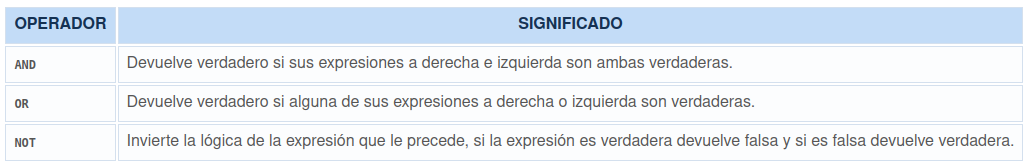
\includegraphics[scale=0.50]{operadores-logicos.png}
    \caption{Operadores lógicos en SQL}
\end{figure}

A continuación vemos dos ejemplos de uso de los operadores lógicos en Oracle y MySQL.

\begin{itemize}
    \item \textbf{Oracle}: si queremos obtener aquellas salas cuya capacidad esté entre 100 y 300 personas sería:

    \begin{figure}[h]
        \begin{tcolorbox}[sharp corners, colback=yellow!30, colframe=white!20]
            \scriptsize
            \begin{verbatim}


                SELECT nombre, capacidad FROM SALA WHERE capacidad>=100 AND capacidad<=300;
            \end{verbatim}
        \end{tcolorbox}
    \end{figure}

    \item \textbf{MySQL}: si queremos obtener aquellos empleados cuyo salario sera menor o igual a 2000€ o superior a 2500€.
\end{itemize}

\subsection{Precedencias}
Con frecuencia utilizaremos la sentencia \textbf{SELECT} con expresiones muy extensas y resultará difícil saber que parte de dicha expresión se evaluará primero. Por ello, es conveniente saber el orden de precedencia de los diferentes operadores que hemos visto. Así, ésto se evaluarán con el siguiente orden:

\begin{enumerate}
    \item Se evalúa la multiplicación (\textbf{*}) y la división (\textbf{/}) al mismo nivel.
    \item A continuación sumas (\textbf{+}) y restas (\textbf{-}).
    \item Concatenación (\textbf{||}) (solo en \textbf{Oracle})
    \item Todas las comparaciones (\textbf{<}, \textbf{>}, ...)
    \item Los operadores \textbf{IS NULL}, \textbf{IS NOT NULL}, \textbf{LIKE} y \textbf{BETWEEN}.
    \item \textbf{NOT}.
    \item \textbf{AND}.
    \item \textbf{OR}.
\end{enumerate}

En el caso de que queramos variar este orden, siempre podemos \textbf{usar paréntesis} para agrupar las expresiones que queremos que se evalúen en primer lugar.

\section{Consultar Calculadas}
En ocasiones es interesante realizar operaciones con algunos campos para obtener información derivada de estos.

Por ejemplo, si tenemos un campo precio, nos podría interesar mostrar los precios con el IVA añadido, o si tuviéramos un campo Sueldo, podríamos mostrar este más la suma de una Paga Extra. Estos son ejemplos simples, pero podemos construir expresiones mucho más complejas. 	Para ello, haremos uso de la \textbf{creación de campos calculados}.

Los \textbf{operadores aritméticos} se pueden emplear para realizar cálculos en las consultas. Estos \textbf{campos calculados} se obtiene haciendo uso de la sentencia \textbf{SELECT} poniendo a continuación la expresión que queramos. Este tipo de consultas, \textbf{no modifica los valores originales}, de las columnas de la tabla/s en la que se esta realizando dicha consulta, unicamente mostrará una nueva columna con los valores calculados. Por ejemplo:

\begin{itemize}
    \item \textbf{Oracle}: podemos crear una columna con el valor de precio + 10, como podemos ver en la siguiente consulta.

    \begin{figure}[h]
        \begin{tcolorbox}[sharp corners, colback=yellow!30, colframe=white!20]
            \scriptsize
            \begin{verbatim}


            SELECT tema, precio, precio + 10 FROM CONFERENCIA;
            \end{verbatim}
        \end{tcolorbox}
    \end{figure}

    También podríamos asignar un alias a la columna para que nos muestre un nuevo nombre en esta, añadiendo \textbf{AS} después de la expresión y el \textbf{nombre del alias}.

        \begin{figure}[h]
        \begin{tcolorbox}[sharp corners, colback=yellow!30, colframe=white!20]
            \scriptsize
            \begin{verbatim}


            SELECT tema, precio, precio + 10 AS PrecioNuevo FROM CONFERENCIA;
            \end{verbatim}
        \end{tcolorbox}
    \end{figure}

    \item \textbf{MySQL}: ahora vamos a crear una nueva columna llamada SalarioNuevo en MySQL:

    \begin{figure}[H]
        \begin{tcolorbox}[sharp corners, colback=yellow!30, colframe=white!20]
            \scriptsize
            \begin{verbatim}


            SELECT nombre, salario, salario + 25 AS SalarioNuevo FROM empleado;
            \end{verbatim}
        \end{tcolorbox}
    \end{figure}
\end{itemize}

\section{Funciones}
En casi todos los sistemas de gestiones de datos existen \textbf{funciones} que nos ayudan a crear consultas más complejas. Dichas funciones varían según el SGBD. Aquí, veremos en concreto las de \textbf{Oracle}.

Las \textbf{funciones} son realmente operaciones que se realizan sobre los datos y que realizan un cálculo determinado. Para ello necesitamos uno datos de entrada, llamados \textbf{parámetros} en función de los cuales se realizarán los cálculos adecuados. Normalmente, estos parámetros se especifican entre paréntesis.

Las funciones se pueden incluir en la cláusulas \textbf{SELECT}, \textbf{WHERE} y \textbf{ORDER BY}.

Las funciones suelen tener la siguiente sintaxis:

\begin{figure}[h]
    \begin{tcolorbox}[sharp corners, colback=yellow!30, colframe=white!20]
        \scriptsize
        \begin{verbatim}


                      NombreFunción (parámetro1, parámetro2, …)
        \end{verbatim}
    \end{tcolorbox}
\end{figure}

Las funciones \textbf{se pueden anidar} unas dentro de otras. Existen, además, una gran variedad de funciones para cada tipo de datos, siendo las principales:

\begin{itemize}
    \item Numéricas.
    \item De cadenas de caracteres.
    \item De manejo de fechas.
    \item De conversión.
    \item etc...
\end{itemize}

\subsection{Funciones Numéricas}
Este tipo de funciones se emplean para trabajar con \textbf{campos numéricos}, permitiéndonos realizar una serie de operaciones sobre este tipo de dato. Las principales funciones de este tipo son las siguientes:

\begin{itemize}
    \item \textbf{ABS(n)}

    Esta función calcula el \textbf{valor absoluto} de un número dado n.

    \begin{itemize}
        \item \textbf{Oracle}:

        \begin{figure}[h]
            \begin{tcolorbox}[sharp corners, colback=yellow!30, colframe=white!20]
                \scriptsize
                \begin{verbatim}


                SELECT ABS(-17) FROM DUAL;

                -- Resultado: 17
                \end{verbatim}
            \end{tcolorbox}
        \end{figure}

         \item \textbf{MySQL}:

            \begin{figure}[h]
        \begin{tcolorbox}[sharp corners, colback=yellow!30, colframe=white!20]
            \scriptsize
            \begin{verbatim}


                SELECT ABS(-17);

                -- Resultado: 17
            \end{verbatim}
        \end{tcolorbox}
    \end{figure}


    \begin{figure}[H]
        \begin{tcolorbox}[sharp corners, colback=cyan!30, colframe=white!20]
            \normalsize

        Observa que con MySQL no es necesario utilizar ninguna tabla. Basta con hacer la SELECT a la función. El resto de ejemplos expuestos funcionan igual. En MySQL los puedes probar sin poner la tabla DUAL.
        \end{tcolorbox}
    \end{figure}
    \end{itemize}

    \item \textbf{EXP(n)}:

    Calcula el \textbf{exponencial}, es decir, exponente en base e, de un número dado n.

     \begin{figure}[H]
        \begin{tcolorbox}[sharp corners, colback=yellow!30, colframe=white!20]
            \scriptsize
            \begin{verbatim}


                SELECT EXP(-17) FROM DUAL;

                -- Resultado: 7.38
            \end{verbatim}
        \end{tcolorbox}
    \end{figure}

    \item \textbf{CEIL(n)}

    Calcula el \textbf{valor entero} inmediatamente \textbf{superior o igual} a n.

    \begin{figure}[H]
        \begin{tcolorbox}[sharp corners, colback=yellow!30, colframe=white!20]
            \scriptsize
            \begin{verbatim}


                SELECT CEIL(17.4) FROM DUAL;

                -- Resultado: 18
            \end{verbatim}
        \end{tcolorbox}
    \end{figure}

      \item \textbf{FLOOR(n)}

      Calcula el \textbf{valor entero} inmediatamente \textbf{inferior o igual} a n.

    \begin{figure}[H]
        \begin{tcolorbox}[sharp corners, colback=yellow!30, colframe=white!20]
            \scriptsize
            \begin{verbatim}


                SELECT FLOOR(17.4) FROM DUAL;

                -- Resultado: 17
            \end{verbatim}
        \end{tcolorbox}
    \end{figure}

    \item \textbf{MOD(n, m)}

    Calcula el \textbf{resto} resultante de \textbf{dividir n entre m}.

    \begin{figure}[H]
        \begin{tcolorbox}[sharp corners, colback=yellow!30, colframe=white!20]
            \scriptsize
            \begin{verbatim}


                SELECT MOD(115, 2) FROM DUAL;

                -- Resultado: 1
            \end{verbatim}
        \end{tcolorbox}
    \end{figure}

    \item \textbf{POWER(n, m)}

    Calcula el valor de \textbf{elevar n} al \textbf{exponente m}.

    \begin{figure}[H]
        \begin{tcolorbox}[sharp corners, colback=yellow!30, colframe=white!20]
            \scriptsize
            \begin{verbatim}


                SELECT POWER(4, 5) FROM DUAL;

                -- Resultado: 1024
            \end{verbatim}
        \end{tcolorbox}
    \end{figure}

    \item \textbf{ROUND(n, decimales)}:

    \textbf{Redondea} el número n al \textbf{siguiente número} con la \textbf{cantidad de decimales} indicada.

    \begin{figure}[H]
        \begin{tcolorbox}[sharp corners, colback=yellow!30, colframe=white!20]
            \scriptsize
            \begin{verbatim}


                SELECT ROUND(12.5876, 2) FROM DUAL;

                -- Resultado: 12.59
            \end{verbatim}
        \end{tcolorbox}
    \end{figure}

      \item \textbf{SQRT(n)}

      Calcula la \textbf{raíz cuadrada} de n.

    \begin{figure}[H]
        \begin{tcolorbox}[sharp corners, colback=yellow!30, colframe=white!20]
            \scriptsize
            \begin{verbatim}


                SELECT SQRT(25) FROM DUAL;

                -- Resultado: 5
            \end{verbatim}
        \end{tcolorbox}
    \end{figure}

    \item \textbf{TRUNC(n, decimales)}:

    \textbf{Trunca} el número n a la \textbf{cantidad de decimales} indicada. Si se omite el segundo argumento, se truncan todos los decimales. Si n es \textbf{negativo}, el número es truncado desde la parte entera.

    \begin{figure}[H]
        \begin{tcolorbox}[sharp corners, colback=yellow!30, colframe=white!20]
            \scriptsize
            \begin{verbatim}


                SELECT TRUNC(127.4567, 2) FROM DUAL;

                -- Resultado: 127.45

                SELECT TRUNC(4572.5678, -2) FROM DUAL;

                -- Resultado: 4500

                SELECT TRUNC(4572.5678, -1) FROM DUAL;

                -- Resultado: 4570

                SELECT TRUNC(4572.5678) FROM DUAL;

                -- Resultado: 4572
            \end{verbatim}
        \end{tcolorbox}
    \end{figure}

    \item \textbf{SIGN(n)}

    Si el parámetro n es un valor \textbf{positivo}, \textbf{devuelve 1}, si es \textbf{negativo}, \textbf{devuelve -1} y si el valor de n \textbf{es 0}, \textbf{devuelve 0}.

    \begin{figure}[H]
        \begin{tcolorbox}[sharp corners, colback=yellow!30, colframe=white!20]
            \scriptsize
            \begin{verbatim}


                SELECT SIGN(-4) FROM DUAL;

                -- Resultado: -1
            \end{verbatim}
        \end{tcolorbox}
    \end{figure}
    \end{itemize}


\subsection{Funciones de Cadena de Caracteres}
Una de las acciones más comunes que realizaremos es la manipulación de campos de tipo carácter o cadena de caracteres. Las principales funciones para este tipo de manipulación son las siguientes:

\begin{itemize}
    \item \textbf{CHR(n)}

    Devuelve el carácter cuyo \textbf{valor codificado} es n.

      \begin{figure}[H]
        \begin{tcolorbox}[sharp corners, colback=yellow!30, colframe=white!20]
            \scriptsize
            \begin{verbatim}


                SELECT CHR(81) FROM DUAL;

                -- Resultado: Q
            \end{verbatim}
        \end{tcolorbox}
    \end{figure}

    \item \textbf{ASCII(n)}

    Devuelve el \textbf{valor ASCII }del carácter n.

    \begin{figure}[H]
        \begin{tcolorbox}[sharp corners, colback=yellow!30, colframe=white!20]
            \scriptsize
            \begin{verbatim}


                SELECT ASCII('O') FROM DUAL;

                -- Resultado: 79
            \end{verbatim}
        \end{tcolorbox}
    \end{figure}

    \item \textbf{CONCAT(cad1, cad2)}

    Devuelve la \textbf{cadena resultante} de \textbf{concatenar} las cadenas cad1 y cad2.

    \begin{figure}[H]
        \begin{tcolorbox}[sharp corners, colback=yellow!30, colframe=white!20]
            \scriptsize
            \begin{verbatim}


                SELECT CONCAT('Hola', 'Mundo') FROM DUAL;

                -- Resultado: HolaMundo
            \end{verbatim}
        \end{tcolorbox}
    \end{figure}

    \item \textbf{LOWer(cad)}

    Devuelve la \textbf{cadena} cad con todos los \textbf{caracteres en minúscula}.

    \begin{figure}[H]
        \begin{tcolorbox}[sharp corners, colback=yellow!30, colframe=white!20]
            \scriptsize
            \begin{verbatim}


                SELECT LOWER('Hola') FROM DUAL;

                -- Resultado: hola
            \end{verbatim}
        \end{tcolorbox}
    \end{figure}

    \item \textbf{UPPER(cad)}

    Devuelve la \textbf{cadena} cad con todos los \textbf{caracteres en mayúscula}.

    \begin{figure}[H]
        \begin{tcolorbox}[sharp corners, colback=yellow!30, colframe=white!20]
            \scriptsize
            \begin{verbatim}


                SELECT UPPER('Hola') FROM DUAL;

                -- Resultado: HOLA
            \end{verbatim}
        \end{tcolorbox}
    \end{figure}

    \item \textbf{INITCAP(cad)}

    Devuelve la \textbf{cadena} cad con el \textbf{primer carácter} en \textbf{mayúsculas}.

    \begin{figure}[H]
        \begin{tcolorbox}[sharp corners, colback=yellow!30, colframe=white!20]
            \scriptsize
            \begin{verbatim}


                SELECT INITCAP('hola') FROM DUAL;

                -- Resultado: Hola
            \end{verbatim}
        \end{tcolorbox}
    \end{figure}
\end{itemize}
% Apéndice
\appendix

% Change appendix display options
\titleformat{\chapter}{\bfseries\Huge}{\thechapter.}{1ex}{}
\chapter{Anexos Tema 4}

\section{Creación de Tablas y Preparación de Oracle y MySQL}
En este apéndice vamos a indicar el proceso para crear las bases de datos que vamos a usar en la unidad 4, tanto en Oracle como en MySQL.

\subsection{Creación de las Tablas en Oracle}
Para la creación de las tablas en el SGBD de Oracle debemos seguir los siguiente pasos:

\begin{enumerate}
    \item En primer lugar crearemos un espacio de trabajo o Workbench llamado \textbf{TAREA} con un usuario llamado \textbf{ANA} al que pondremos también la contraseña que queramos. Este usuario será por tanto el administrador de este espacio de trabajo y tendrá permisos para crear tablas.

    \begin{figure}[H]
        \centering
        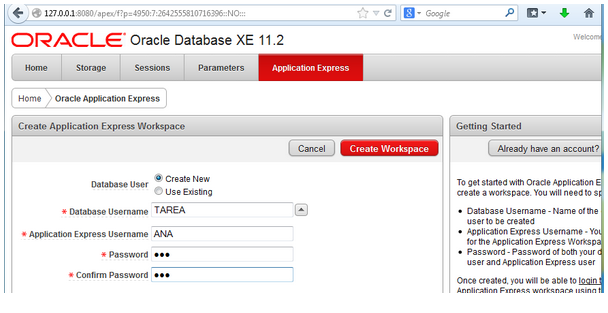
\includegraphics[scale=0.80]{creacion-oracle-1.png}
        \caption{Creación del espacio de trabajo y el usuario}
    \end{figure}

    \item A continuación, vamos a descargar el archivo con el \textbf{script sql} para la creación de tablas. El archivo podemos encontrarlo \href{https://github.com/fcosueza/DAW/blob/main/BD/Apuntes/archivos/tema4-script-oracle.zip}{este enlace}  de github, y pulsando en \textbf{download} lo descargamos.

    Una vez descargado, vamos a utilizar la \textbf{línea de comandos de SQL} para ejecutar el archivo descargado. Para acceder a la línea de comandos debemos hacer lo siguiente:

    \begin{enumerate}
        \item Vamos a \textbf{Inicio > Todos los Programas > Oracle Database 11g Express Edition}.
        \item Pulsando en \textbf{Run SQL Command Line} aparecerá la siguiente pantalla:

        \begin{figure}[H]
            \centering
            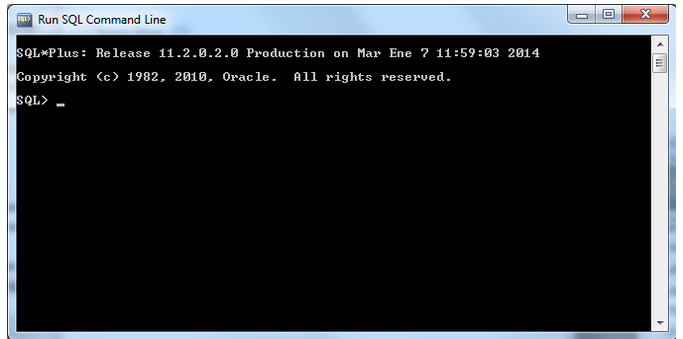
\includegraphics[scale=0.50]{creacion-oracle-2.png}
            \caption{Línea de comandos de SQL en Oracle}
        \end{figure}
    \end{enumerate}

    \item Una vez abierta la línea de comandos de SQL, debemos ejecutar la instrucción \textbf{connect TAREA\textbackslash ANA}, que corresponde al espacio de trabajo creado anteriormente con la contraseña del usuario administrador en mayúsculas.

    \begin{figure}[H]
        \centering
        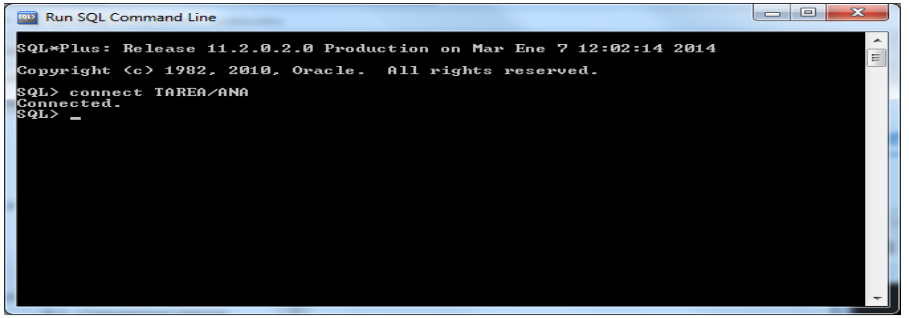
\includegraphics[scale=0.40]{creacion-oracle-3.png}
        \caption{Conexión al espacio de trabajo creado}
    \end{figure}

    Una vez ejecutada la instrucción, si se ha realizado correctamente, se nos mostrará el mensaje \textbf{Connected}, indicándonos que se ha realizado la conexión.

    \item Una vez realizada la conexión, podemos proceder a ejecutar el archivo descargado anteriormente, indicándolo del de la siguiente manera: \textbf{@ruta\_archivo/BD04\_CONT\_R07\_02.sql}, como se muestra en la siguiente captura.

    \begin{figure}[H]
        \centering
        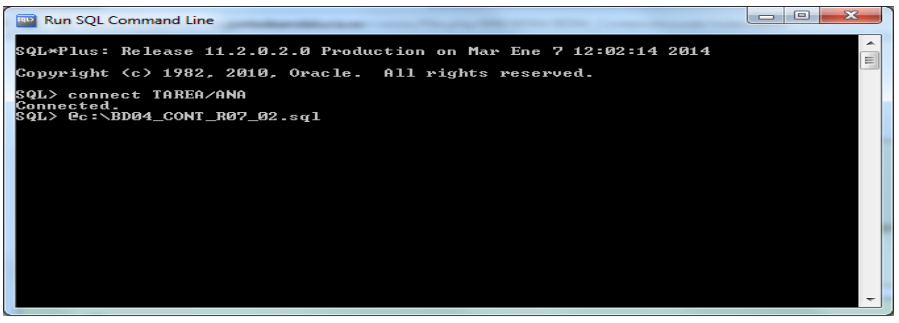
\includegraphics[scale=0.40]{creacion-oracle-4.png}
        \caption{Ejecución del script proporcionado}
    \end{figure}

    Si todo se ha realizado correctamente, la aplicación nos mostrará un mensaje \textbf{Table created}, por cada tabla nueva que se haya creado, así como una mensaje  \textbf{1 row created} por cada dato creado.

    \item Por último, ya solo nos queda desconectar de la base de datos para poder consultar las tablas y datos creados desde la aplicación gráfica. Para ello, introducimos el comando \textbf{DISCONNECT} y pulsamos \textbf{Enter}.

    \begin{figure}[H]
        \centering
        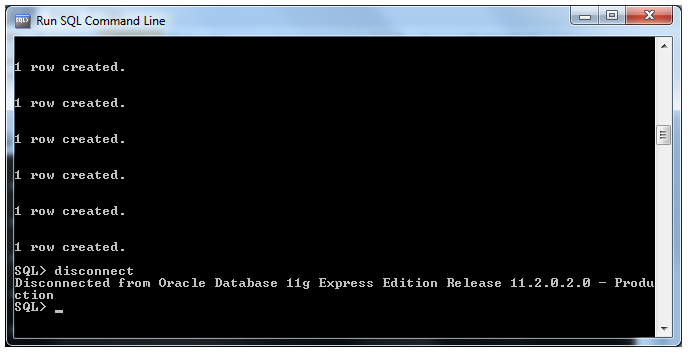
\includegraphics[scale=0.45]{creacion-oracle-5.png}
        \caption{Desconexión de la base de datos}
    \end{figure}
\end{enumerate}

\subsection{Creación de las Tablas en MySQL}
Ahora vamos a ver como realizar el mismo procedimiento para crear la base de datos necesaria para este tema en MySQL.

\begin{enumerate}
    \item En primer lugar vamos a descargar el \textbf{script} para \textbf{generar las tablas} en MySQL, el cual podemos encontrar en \href{https://github.com/fcosueza/DAW/blob/main/BD/Apuntes/archivos/tema4-script-mysql.zip}{este enlace}. Una vez descargado el script, iniciamos sesión en nuestro servido MySQL. Para ello, asegúrate de tener iniciado el servidor  de bases de datos MySQL e inicia sesión como el usuario \textbf{root}, indicando su contraseña.

    \begin{figure}[H]
        \centering
        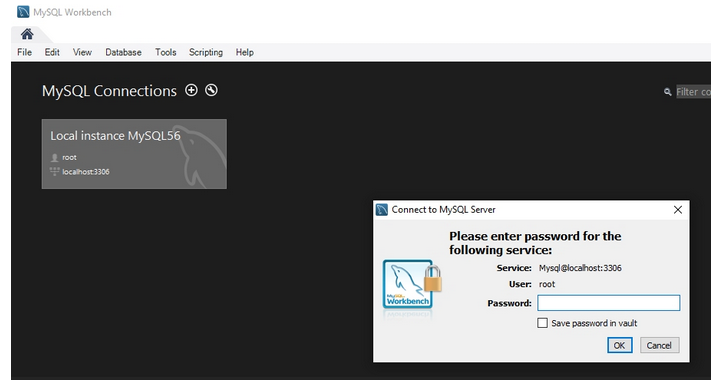
\includegraphics[scale=0.45]{creacion-mysql-1.png}
        \caption{Inicio de sesión en el servidor MySQL}
    \end{figure}

    \item El siguiente paso es cargar el script, \textbf{bd\_proyectosx.sql}, que hemos descargado anteriormente. Para ello, pulsamos en la opción \textbf{File > Open SQL Script...} en el menú de Workbench y buscamos el archivo en nuestras carpetas. Lo seleccionamos y al pulsar \textbf{Abrir} el script aparecerá en pantalla.

    \begin{figure}[H]
        \centering
        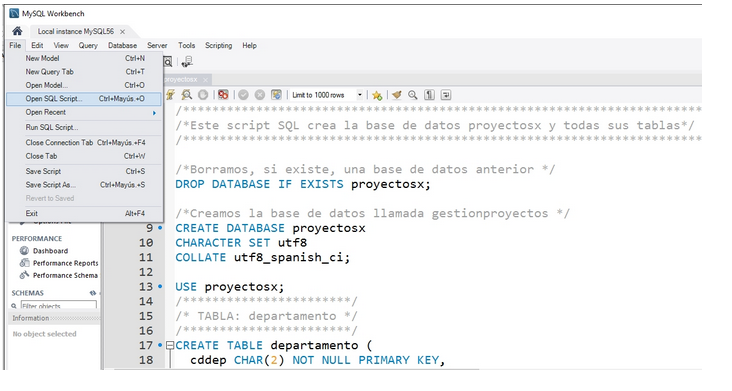
\includegraphics[scale=0.42]{creacion-mysql-2.png}
        \caption{Carga del script en MySQL Workbench}
    \end{figure}

    \item Con el script ya cargado y en pantalla, pulsamos sobre \textbf{File > Run SQL Script} o bien en el icono de un ``\textbf{rayo amarillo}''. Una vez realizado esto, el script se ejecutara y la base de datos quedará implantada.

    \begin{figure}[H]
        \centering
        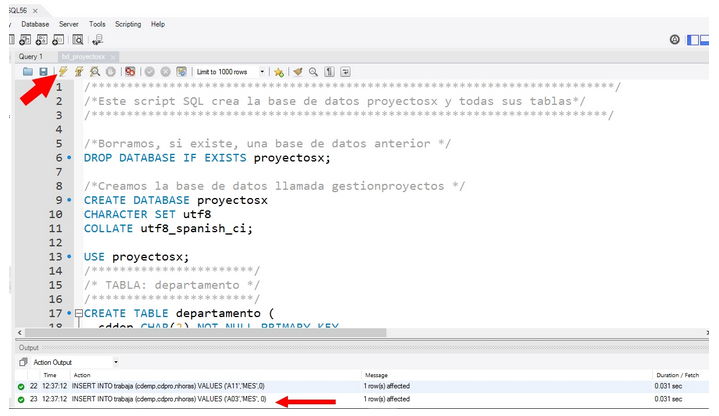
\includegraphics[scale=0.50]{creacion-mysql-3.png}
        \caption{Ejecución del script y creación de la base de datos}
    \end{figure}

    \item Ya solo tenemos que actualiza la información en lista de la izquierda de Workbench pulsando en el \textbf{icono de las dos flechas} o pulsando con el botón derecho sobre ese menú y seleccionando \textbf{Refresh All}, para que así se nos muestre la nueva base de datos creada.

    \begin{figure}[H]
        \centering
        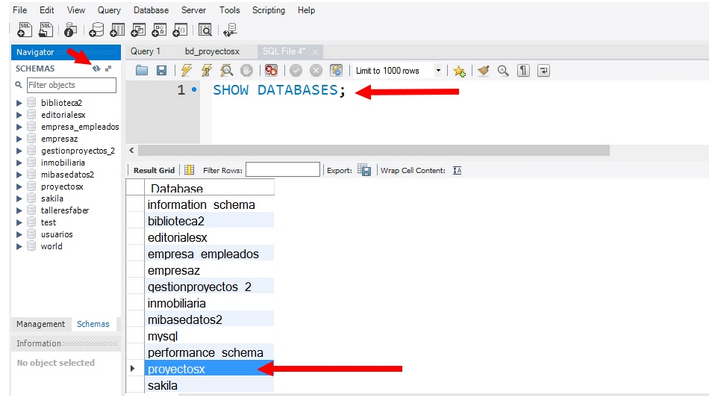
\includegraphics[scale=0.45]{creacion-mysql-4.png}
        \caption{Actualización de la lista de bases de datos en Workbench}
    \end{figure}
\end{enumerate}

Tras estos pasos, ya tendremos nuestra base de datos creada en el servidor MySQL. Si queremos podemos mostrar las bases de datos que este tiene usando la sentencia \textbf{SHOW databases}, o realizar algunas consultas genéricas, como \textbf{SELECT * from empleados}, para comprobar los diferentes elementos que tiene cada tabla.


% Glossary

\glsaddall
\printglossaries

% Bibliography

\newpage
\addcontentsline{toc}{chapter}{Bibliografía}
\bibliography{citas}
\bibliographystyle{unsrt}

\end{document}